\documentclass[11pt,a4paper]{article}
\usepackage[margin=1in]{geometry}
\usepackage[T1]{fontenc}
\usepackage{lmodern}
\usepackage{amsmath,amssymb,amsthm,mathtools}
\usepackage{booktabs,array}
\usepackage{enumitem}
\usepackage{tikz}
\usetikzlibrary{arrows.meta,positioning,calc,fit}
\usepackage[hidelinks]{hyperref}

\setlength{\parindent}{0pt}
\emergencystretch=3em
\setlength{\parskip}{0.7em}
\setlist{itemsep=0.2em,topsep=0.3em}

\theoremstyle{definition}
\newtheorem{definition}{Definition}[section]
\newtheorem{theorem}[definition]{Theorem}
\newtheorem{example}[definition]{Example}
\newtheorem{remark}[definition]{Remark}

\newcommand{\Z}{\mathbb{Z}}
\newcommand{\F}{\mathbb{F}}
\newcommand{\Gen}{\mathsf{Gen}}
\newcommand{\Sign}{\mathsf{Sign}}
\newcommand{\Ver}{\mathsf{Ver}}
\newcommand{\sk}{\mathit{sk}}
\newcommand{\pk}{\mathit{pk}}
\newcommand{\Hash}{H}
\newcommand{\HB}{\mathsf{HighBits}}
\newcommand{\norm}[1]{\lVert #1\rVert}
\newcommand{\inv}[1]{#1^{-1}}

\tikzset{
  actor/.style={draw,rounded corners=2pt,minimum width=2.2cm,minimum height=0.8cm,fill=gray!10,font=\small},
  box/.style={draw,rounded corners=2pt,fill=white,font=\footnotesize,align=center,inner sep=3pt},
  msg/.style={-{Stealth[length=2.5mm]},thick},
  life/.style={dashed,gray}
}

\title{Digital Signatures\\[0.3em]\large From RSA to Bitcoin to Lattices}
\author{Lecture Notes}
\date{}

\begin{document}
\maketitle
\tableofcontents
\bigskip

\setcounter{section}{-1}

%=====================================================================
\section{Why Digital Signatures?}
%=====================================================================

\subsection{What encryption does not give}

Encryption answers one question: who is allowed to read a message. A message encrypted for Bob is unreadable to everybody else, and that is all it promises. It says nothing about who wrote the message, and it does not promise that the message arrives unchanged. The following situations show the gap.

Suppose Alice banks with Bob. Bob's bank publishes its public encryption key $\pk_B$ so that customers can send private instructions. Oscar, who wants Alice's money, reads the public key from the bank's website and computes
\[
c = \mathsf{Enc}(\pk_B,\ \text{``Transfer 100 from Alice's account to Oscar''}).
\]
The bank decrypts $c$ and finds a perfectly well-formed instruction. Nothing in the ciphertext reveals who produced it, because the encryption key is public and anybody can use it. Public-key encryption gives Bob confidentiality but no information about the sender.

Symmetric encryption looks better at first. If Alice and Bob share a secret key $K$, then Oscar cannot create a fresh ciphertext of his own choosing. Two problems remain. The first is that many ciphers can be modified without the key.

\begin{example}[Bit flipping in a stream cipher]\label{ex:bitflip}
Alice sends Bob the amount ``100'' encrypted with a stream cipher, which XORs the ASCII bytes of the plaintext with a secret keystream $k$. The ASCII code of the character \texttt{1} is $0\mathrm{x}31 = 00110001_2$ and the code of \texttt{9} is $0\mathrm{x}39 = 00111001_2$. These two bytes differ in exactly one bit, namely the bit with value $8$, so $0\mathrm{x}31 \oplus 0\mathrm{x}39 = 0\mathrm{x}08$.

Oscar does not know the keystream. He knows that the amount in the message is ``100'', so the first byte of the ciphertext is $c_1 = 0\mathrm{x}31 \oplus k_1$. He replaces $c_1$ by $c_1' = c_1 \oplus 0\mathrm{x}08$. Bob decrypts
\[
c_1' \oplus k_1 = 0\mathrm{x}31 \oplus k_1 \oplus 0\mathrm{x}08 \oplus k_1 = 0\mathrm{x}39 = \texttt{9},
\]
and reads ``900''. The ciphertext was altered, the alteration was invisible, and the key was never needed.
\end{example}

The second problem is that a shared key cannot settle a dispute. If Bob later claims that Alice sent ``Transfer 900'', Alice can say that Bob wrote the message himself, since Bob holds the same key. A judge looking at the evidence cannot tell the two stories apart.

\subsection{The services a signature provides}

A digital signature is a short piece of data $\sigma$ that is computed from a message $m$ and a secret key, and that anybody can check against a public key. A valid signature gives the following services.

\textbf{Integrity.} If a single bit of $m$ changes after signing, the signature no longer verifies. The receiver learns that the message is exactly the one that was signed.

\textbf{Data-origin authentication.} Only the holder of the secret key can produce a valid signature, so a valid signature ties the message to the owner of the matching public key.

\textbf{Non-repudiation.} Alice cannot later deny having signed $m$, because nobody else holds her secret key. This is the service that a shared-key mechanism can never give.

\textbf{Public verifiability.} Verification needs only the public key. Bob can forward $(m,\sigma)$ to a judge, to a newspaper or to the whole Bitcoin network, and every one of them can check it without any secret.

A message authentication code (MAC) sits between encryption and signatures. It gives integrity and authentication, but only between two parties who share the key, and it gives neither non-repudiation nor public verifiability. Table~\ref{tab:services} puts the three tools side by side.

\begin{table}[h]
\centering
\begin{tabular}{lccc}
\toprule
 & Encryption & MAC & Signature\\
\midrule
Confidentiality & yes & no & no\\
Integrity & no (malleable) & yes & yes\\
Origin authentication & no & only to the partner & to everyone\\
Non-repudiation & no & no & yes\\
Verifier needs a secret & --- & yes (shared key) & no\\
\bottomrule
\end{tabular}
\caption{What each tool provides. A system that needs both secrecy and authenticity combines encryption with a signature or a MAC.}\label{tab:services}
\end{table}

\begin{example}[A dispute]\label{ex:dispute}
Alice and Bob exchange orders protected by a MAC with shared key $K$. One day Bob presents the order ``PAY BOB 900'' together with a correct MAC tag and demands payment. Alice replies that she only ever sent ``PAY BOB 100''. Both parties are able to compute valid tags under $K$, so the judge has no way to tell who is lying.

Now suppose the same orders are signed. Alice's signing key never leaves her device, so Bob cannot produce a valid signature on ``PAY BOB 900''. If Bob presents one, the judge checks it with Alice's public key and concludes that Alice signed it. If Bob cannot present one, his claim fails. The signature settles the dispute in a way that no shared key can.
\end{example}

\subsection{Definition of a signature scheme}

\begin{definition}[Digital signature scheme]
A digital signature scheme consists of three algorithms.
\begin{itemize}
\item $\Gen(1^\lambda)$ takes a security parameter and outputs a key pair $(\pk,\sk)$. The public key $\pk$ is published and the secret key $\sk$ stays with the signer.
\item $\Sign(\sk, m)$ outputs a signature $\sigma$ on the message $m$.
\item $\Ver(\pk, m, \sigma)$ outputs \textsf{accept} or \textsf{reject}.
\end{itemize}
The scheme is \emph{correct} if $\Ver(\pk, m, \Sign(\sk,m)) = \textsf{accept}$ for every key pair and every message.
\end{definition}

In plain words, the signer uses the secret key to sign, everybody else uses the public key to verify, and honestly produced signatures always pass.

Correctness is not enough, because a scheme that accepts every pair $(m,\sigma)$ is correct and useless. Security asks that signatures cannot be forged. The standard notion is the following game, called existential unforgeability under chosen-message attack (EUF-CMA). The attacker Eve receives $\pk$. She may ask the signer for signatures on any messages she likes, as many as she wants. She wins if she outputs a pair $(m^*,\sigma^*)$ that verifies and in which $m^*$ is a message the signer was never asked to sign. The scheme is secure if no efficient Eve wins with noticeable probability. The word ``existential'' means that Eve wins even if $m^*$ is meaningless text, because a meaningless-looking bit string can turn out to encode a valid order in some other context.

\begin{example}[Winning the game]
Alice's signer has produced signatures on ``PAY BOB 100'' and ``PAY CAROL 50''. If Eve outputs ``PAY BOB 100'' with its signature, she has won nothing, since this message was already signed. If she outputs a valid signature on the new message ``PAY EVE 100'', or even on the random string ``q7\#xw'', she has produced an existential forgery and the scheme is broken.
\end{example}

\subsection{Hash-and-sign}

Signature algorithms work on numbers of a fixed size, whereas messages can be megabytes long. Every practical scheme therefore signs a short fingerprint $h = \Hash(m)$ of the message, where $\Hash$ is a collision-resistant hash function such as SHA-256. The verifier recomputes the hash and checks the signature against it. Collision resistance is essential: if Eve could find two messages $m \neq m'$ with $\Hash(m)=\Hash(m')$, then a signature on $m$ would also be a valid signature on $m'$. Hashing also destroys the algebraic structure that attacks on ``raw'' schemes exploit, as Section~1 shows.

\begin{figure}[h]
\centering
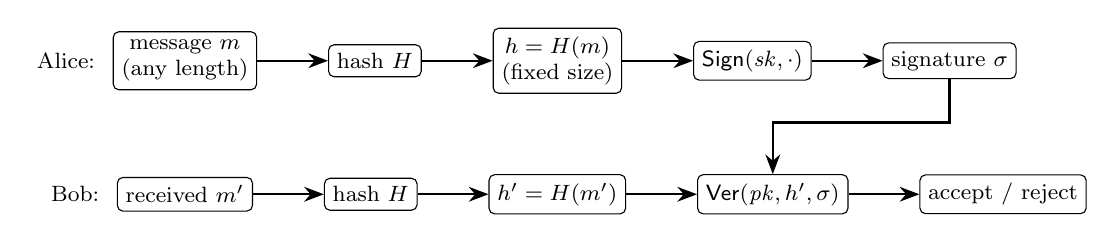
\begin{tikzpicture}[node distance=0.9cm]
\node[box] (m) {message $m$\\(any length)};
\node[box,right=of m] (h) {hash $\Hash$};
\node[box,right=of h] (d) {$h=\Hash(m)$\\(fixed size)};
\node[box,right=of d] (s) {$\Sign(\sk,\cdot)$};
\node[box,right=of s] (sig) {signature $\sigma$};
\draw[msg] (m)--(h); \draw[msg] (h)--(d); \draw[msg] (d)--(s); \draw[msg] (s)--(sig);
\node[box,below=1.1cm of m] (m2) {received $m'$};
\node[box,right=of m2] (h2) {hash $\Hash$};
\node[box,right=of h2] (d2) {$h'=\Hash(m')$};
\node[box,right=of d2] (v) {$\Ver(\pk,h',\sigma)$};
\node[box,right=of v] (acc) {accept / reject};
\draw[msg] (m2)--(h2); \draw[msg] (h2)--(d2); \draw[msg] (d2)--(v); \draw[msg] (v)--(acc);
\draw[msg] (sig.south) -- ++(0,-0.55) -| (v.north);
\node[left=0.1cm of m,font=\footnotesize] {Alice:};
\node[left=0.1cm of m2,font=\footnotesize] {Bob:};
\end{tikzpicture}
\caption{Hash-and-sign. Alice signs the hash of the message and Bob checks the signature against the hash of whatever message he received.}
\end{figure}

\subsection{The roles of the keys, and where trust comes from}

Encryption and signatures both use a key pair, but the roles are reversed. To encrypt, anybody uses the public key and only the owner can decrypt with the secret key. To sign, only the owner uses the secret key and anybody can verify with the public key. In the case of RSA the two operations look like mirror images, which has led to the common phrase ``a signature is encryption with the private key''. The phrase is a useful memory aid but a poor description, because real signature schemes hash first, add padding, and for most other schemes (Schnorr, ECDSA, lattices) there is no encryption operation to run backwards at all.

One question remains: how does Bob know that a given public key really belongs to Alice? In practice a certificate authority signs the statement ``this public key belongs to Alice'', and Bob checks that signature with the authority's public key, which his software ships with. Signatures therefore also create trust chains, which Section~4 develops. They protect web connections (TLS certificates), software updates, passports, signed e-mail, and, as Section~2 shows, the ownership of every coin on the Bitcoin network.

\begin{figure}[h]
\centering
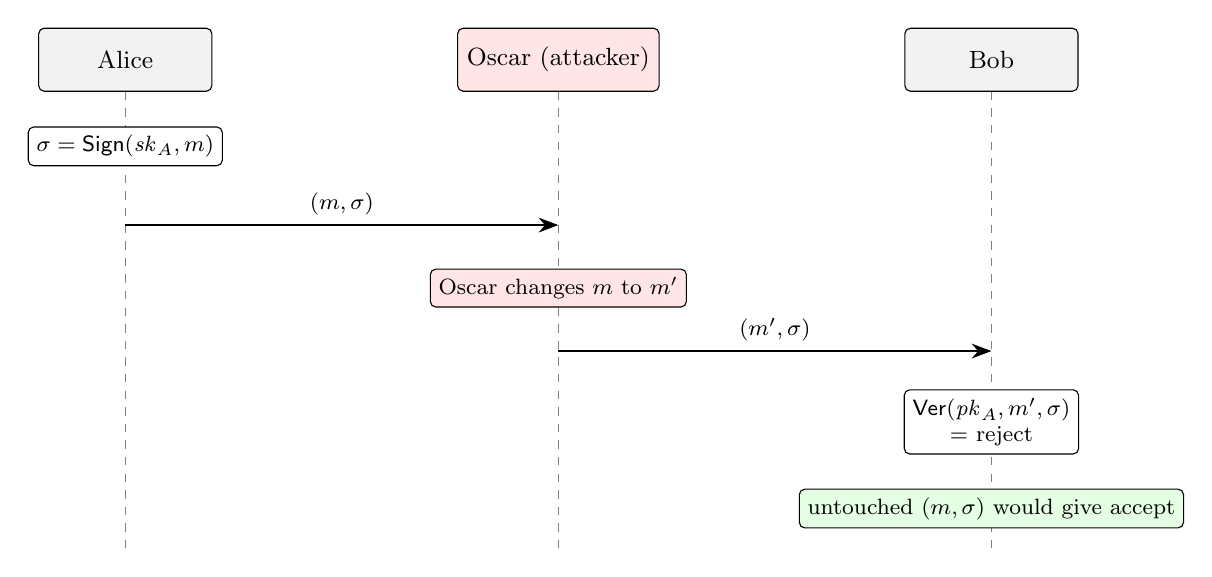
\begin{tikzpicture}[x=1cm,y=1cm]
\node[actor] (A) at (0,0) {Alice};
\node[actor,fill=red!10] (O) at (5.5,0) {Oscar (attacker)};
\node[actor] (B) at (11,0) {Bob};
\draw[life] (A) -- (0,-6.2); \draw[life] (O) -- (5.5,-6.2); \draw[life] (B) -- (11,-6.2);
\node[box] at (0,-1.1) {$\sigma=\Sign(\sk_A,m)$};
\draw[msg] (0,-2.1) -- (5.5,-2.1) node[midway,above,font=\footnotesize] {$(m,\sigma)$};
\node[box,fill=red!10] at (5.5,-2.9) {Oscar changes $m$ to $m'$};
\draw[msg] (5.5,-3.7) -- (11,-3.7) node[midway,above,font=\footnotesize] {$(m',\sigma)$};
\node[box] at (11,-4.6) {$\Ver(\pk_A,m',\sigma)$\\$=$ reject};
\node[box,fill=green!10] at (11,-5.7) {untouched $(m,\sigma)$ would give accept};
\end{tikzpicture}
\caption{Alice signs, Oscar tampers on the way, Bob rejects. Oscar cannot repair $\sigma$ without Alice's secret key.}
\end{figure}

%=====================================================================
\section{RSA Signatures}
%=====================================================================

\subsection{The idea}

RSA is built on a trapdoor: with the public numbers $(n,e)$ anybody can compute $x \mapsto x^e \bmod n$, but undoing this map requires the secret exponent $d$, which in turn requires the factorization of $n$. For encryption the public map hides the message. For signatures the roles are turned around. Alice applies the hard-to-compute direction $h \mapsto h^d \bmod n$ to the hash of her message, and Bob applies the easy direction $s \mapsto s^e \bmod n$ to see whether he gets the hash back. Only Alice can produce an $s$ with $s^e \equiv h$, because only she can compute $e$-th roots modulo $n$.

\subsection{The scheme}

\begin{definition}[RSA signature scheme, textbook form with hashing]
\emph{Key generation.} Choose two large distinct primes $p,q$ and set $n=pq$ and $\varphi(n)=(p-1)(q-1)$. Choose $e$ with $\gcd(e,\varphi(n))=1$ and compute $d \equiv \inv{e} \pmod{\varphi(n)}$. The public key is $\pk=(n,e)$ and the secret key is $\sk=(n,d)$.

\emph{Signing.} For a message $m$ compute $h=\Hash(m)$ with $0\le h<n$ and output $s = h^{d} \bmod n$.

\emph{Verification.} Given $(m,s)$ compute $h=\Hash(m)$ and $h' = s^{e} \bmod n$. Accept if and only if $h'=h$.
\end{definition}

\begin{theorem}[Correctness]
If $s = h^d \bmod n$ then $s^e \equiv h \pmod n$.
\end{theorem}
\begin{proof}
Since $ed\equiv 1 \pmod{\varphi(n)}$ there is an integer $k$ with $ed=1+k(p-1)(q-1)$, and $s^e\equiv h^{ed} \pmod n$. Consider this modulo $p$. If $p\mid h$, then $h^{ed}$ and $h$ are both $0$ modulo $p$. Otherwise Fermat's little theorem gives $h^{p-1}\equiv 1 \pmod p$, so $h^{ed}=h\cdot\big(h^{p-1}\big)^{k(q-1)}\equiv h \pmod p$. The same argument works modulo $q$. Since $p$ and $q$ are distinct primes, the Chinese remainder theorem gives $h^{ed}\equiv h \pmod n$.
\end{proof}

\begin{figure}[h]
\centering
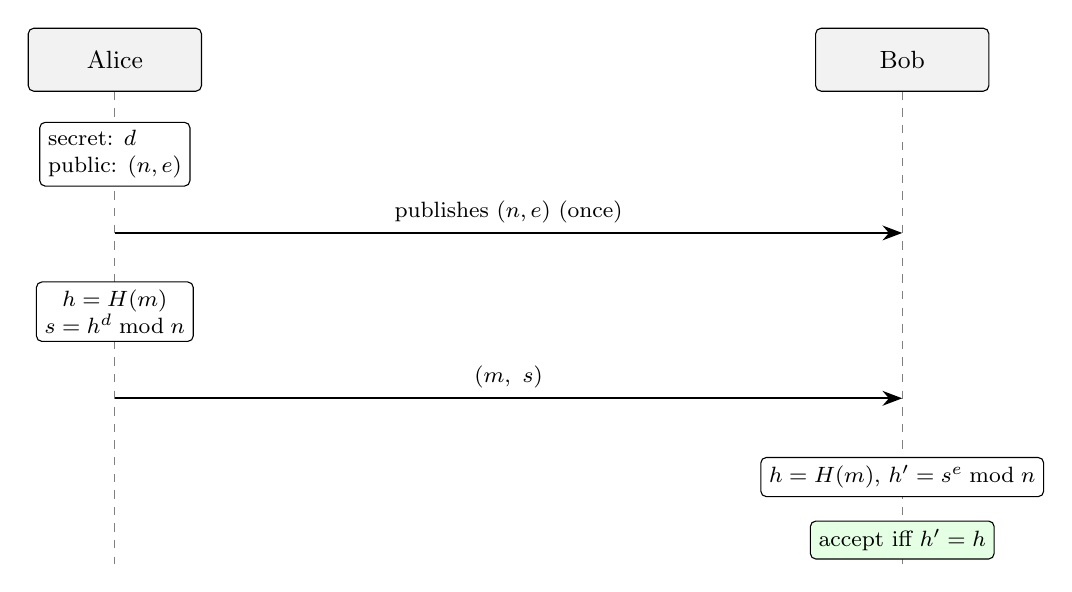
\begin{tikzpicture}[x=1cm,y=1cm]
\node[actor] (A) at (0,0) {Alice};
\node[actor] (B) at (10,0) {Bob};
\draw[life] (A) -- (0,-6.4); \draw[life] (B) -- (10,-6.4);
\node[box,align=left] at (0,-1.2) {secret: $d$\\public: $(n,e)$};
\draw[msg] (0,-2.2) -- (10,-2.2) node[midway,above,font=\footnotesize] {publishes $(n,e)$ (once)};
\node[box] at (0,-3.2) {$h=\Hash(m)$\\$s=h^d \bmod n$};
\draw[msg] (0,-4.3) -- (10,-4.3) node[midway,above,font=\footnotesize] {$(m,\ s)$};
\node[box] at (10,-5.3) {$h=\Hash(m)$, $h'=s^e \bmod n$};
\node[box,fill=green!10] at (10,-6.1) {accept iff $h'=h$};
\end{tikzpicture}
\caption{The interaction in an RSA signature. Only the final message $(m,s)$ travels from Alice to Bob; the key is published once.}
\end{figure}

\subsection{A worked example}

All numbers are tiny so that every step can be followed by hand. Real RSA uses moduli of 2048 bits or more.

\begin{example}[Key generation]\label{ex:rsakey}
Take $p=61$ and $q=53$. Then $n=3233$ and $\varphi(n)=60\cdot 52=3120$. Choose $e=17$, which is coprime to $3120$. The secret exponent is $d=\inv{17} \bmod 3120$. Since $17\cdot 2753 = 46801 = 15\cdot 3120 + 1$, we get $d=2753$. So
\[
\pk=(3233,\,17),\qquad \sk=(3233,\,2753).
\]
\end{example}

\begin{example}[Signing]\label{ex:rsasign}
Let the message be $m=\text{``PAY BOB 100''}$. A real scheme would use SHA-256. For this example we use the toy hash $\Hash(m)=(\text{sum of the ASCII codes of } m) \bmod 3233$. The codes are $80,65,89,32,66,79,66,32,49,48,48$, which add up to $654$, so
\[
h = \Hash(m) = 654.
\]
Alice computes $s = 654^{2753} \bmod 3233$. Computing a power with a large exponent is done by repeated squaring, but a faster way that real implementations use is the Chinese remainder theorem. Alice knows $p$ and $q$, so she reduces the exponent modulo $p-1=60$ and $q-1=52$:
\begin{align*}
d_p &= 2753 \bmod 60 = 53, & d_q &= 2753 \bmod 52 = 49,\\
s_p &= 654^{53} \bmod 61 = 2, & s_q &= 654^{49} \bmod 53 = 27.
\end{align*}
She recombines with Garner's formula. With $q^{-1} \bmod 61 = 38$,
\[
t = 38\,(s_p - s_q) \bmod 61 = 38\cdot(-25) \bmod 61 = 26,\qquad s = s_q + 53\,t = 27 + 1378 = 1405.
\]
The signature is $s=1405$, and Alice sends $(m,s)=(\text{``PAY BOB 100''},\,1405)$ to Bob.
\end{example}

\begin{example}[Verification]\label{ex:rsaver}
Bob computes $h=\Hash(m)=654$ himself, and then $s^e=1405^{17} \bmod 3233$. Since $17=16+1$, he squares four times and multiplies once:
\[
1405^{2}\equiv 1895,\quad 1405^{4}\equiv 2395,\quad 1405^{8}\equiv 683,\quad 1405^{16}\equiv 937 \pmod{3233},
\]
\[
1405^{17} = 1405^{16}\cdot 1405 \equiv 937\cdot 1405 \equiv 654 \pmod{3233}.
\]
The result equals $h=654$, so Bob accepts. Verification is cheap because $e=17$ is small; real keys use $e=65537$.
\end{example}

\begin{example}[A tampered message is rejected]\label{ex:rsatamper}
Oscar changes the message to $m'=\text{``PAY BOB 900''}$ and keeps $s=1405$. Bob hashes the received message and gets $\Hash(m')=662$. He computes $s^e \bmod n = 654$ as before. Since $654\ne 662$, Bob rejects. To make Bob accept, Oscar would have to find $s'$ with $s'^{17}\equiv 662 \pmod{3233}$, which means computing a $17$-th root modulo $n$, and that is exactly what he cannot do without $d$.
\end{example}

\subsection{Why the hash is not optional}

Signing the raw message, $s=m^d \bmod n$, is called textbook RSA, and it is insecure. The reason is that the map $m\mapsto m^d$ has algebraic structure that an attacker can use without knowing $d$. Two attacks illustrate the problem with the numbers from above.

\begin{example}[Existential forgery]\label{ex:rsaforge}
Oscar does not choose a message first. He picks any number he likes as a ``signature'', say $s=1234$, and computes $m = s^e \bmod n = 1234^{17} \bmod 3233 = 2183$. Then $(2183,\,1234)$ passes verification, since $1234^{17}\equiv 2183$. Oscar has produced a valid signature on a message he could not choose, without knowing $d$. If messages are not hashed, ``2183'' might well be interpreted as a meaningful instruction.
\end{example}

\begin{example}[Multiplicative forgery]\label{ex:rsamult}
Signatures are multiplicative because $(m_1 m_2)^d = m_1^d m_2^d$. Suppose Alice has signed $m_1=7$ and $m_2=11$ and the signatures are $s_1=2667$ and $s_2=804$. Oscar multiplies,
\[
s_1 s_2 = 2667\cdot 804 \equiv 789 \pmod{3233},
\]
and $789$ is a valid signature on $m_1m_2=77$. Indeed $77^{2753} \bmod 3233 = 789$. Alice never signed $77$.
\end{example}

Hashing breaks both attacks. In Example~\ref{ex:rsaforge}, Oscar would need a message whose hash equals $2183$, which means inverting the hash function. In Example~\ref{ex:rsamult}, there is no relation between $\Hash(m_1)\Hash(m_2)$ and $\Hash(m_1m_2)$. In practice the hash is not simply reduced modulo $n$ but is expanded and padded to the full size of $n$. The two standard encodings are PKCS\#1 v1.5 and RSA-PSS, and PSS adds a random salt and comes with a security proof in the random oracle model. Real deployments use $|n|\ge 2048$ bits, and the same RSA key pair should never be used for both signing and decryption.

\begin{remark}[Security]
Forging an RSA signature is at least as easy as computing $e$-th roots modulo $n$ (the RSA problem), and recovering $d$ from $(n,e)$ is as hard as factoring $n$. For properly encoded signatures, forgery is believed to be as hard as the RSA problem. Shor's quantum algorithm factors $n$ in polynomial time, so a large quantum computer would break RSA signatures completely, which is one motivation for Section~3.
\end{remark}

%=====================================================================
\section{Bitcoin Signatures: ECDSA and Schnorr}
%=====================================================================

\subsection{The family and the names}

Bitcoin signs transactions with the \emph{Elliptic Curve Digital Signature Algorithm (ECDSA)}, a scheme whose security rests on the discrete logarithm problem. Since the Taproot upgrade of November 2021 Bitcoin also accepts \emph{Schnorr signatures} (specified in BIP~340), which are based on the same problem and are simpler. BIP~340 is a variant of the scheme of Section~\ref{sec:schnorr} with $32$-byte public keys. Both belong to one family. ElGamal (1985) introduced signatures based on discrete logarithms, Schnorr (1989) simplified the idea, and the US standard DSA (1991--1994) re-packaged it to avoid the Schnorr patent. ECDSA is DSA carried over from the group $\Z_p^*$ to the group of points of an elliptic curve, where the same security level needs much shorter keys. Bitcoin uses a specific curve called \texttt{secp256k1}, given by $y^2=x^3+7$ over the field $\F_p$ with $p = 2^{256}-2^{32}-977$. It has a fixed base point $G$ whose order $n \approx 2^{256}$ is prime.

\subsection{The discrete logarithm problem}

\begin{definition}[Discrete logarithm problem]
Let $\mathbb{G}$ be a cyclic group of prime order $n$ with generator $g$. Given $y=g^x$, find $x$. In additive notation, which is used for elliptic curves, the generator is written $G$ and the problem reads: given $Q=dG$, find $d$.
\end{definition}

The forward direction, computing $y=g^x$ from $x$, is fast. The backward direction, finding $x$ from $y$, has no known efficient algorithm in a well-chosen group. This asymmetry lets Alice publish $y$ and keep $x$ secret.

\begin{example}[A tiny discrete logarithm]\label{ex:dlp}
In $\Z_{23}^*$ the element $g=2$ has order $11$, since $2^{11}=2048\equiv 1 \pmod{23}$. Its powers are
\[
2^1,\dots,2^{11} \equiv 2,\ 4,\ 8,\ 16,\ 9,\ 18,\ 13,\ 3,\ 6,\ 12,\ 1 \pmod{23}.
\]
If Alice's public value is $y=18$, anyone can find $x$ with $2^x\equiv 18$ by reading the list: $x=6$. With $11$ possible exponents the search is instant. With a group of order $2^{256}$ the list cannot be written down.
\end{example}

In the group $\Z_p^*$ there are subexponential algorithms for the discrete logarithm (index calculus), so $p$ must have at least $2048$ bits for a modern security level. For the group of points of a suitably chosen elliptic curve only generic algorithms are known, which need about $\sqrt{n}$ steps, and a $256$-bit group already gives $128$ bits of security. This is why Bitcoin, and most modern protocols that rely on the discrete logarithm, work with elliptic curves.

\subsection{Elliptic curves over prime fields}

An elliptic curve is the set of solutions $(x,y)$ of a cubic equation, together with one extra point. The remarkable fact is that the points of such a curve can be \emph{added}, and that this addition behaves like the addition of numbers: it is commutative, has a neutral element, and every point has an inverse. The points then form a group, and the group is what the discrete logarithm problem needs.

\begin{definition}[Elliptic curve over a prime field]
Let $p>3$ be a prime. The elliptic curve $E$ over $\F_p$ is the set of all pairs $(x,y)\in\F_p^2$ that satisfy
\[
y^2\equiv x^3+ax+b \pmod p,
\]
together with an imaginary point $\mathcal{O}$ called the \emph{point at infinity}, where $a,b\in\F_p$ and $4a^3+27b^2\not\equiv 0 \pmod p$.
\end{definition}

The condition $4a^3+27b^2\not\equiv 0$ guarantees that the curve has no cusps and no self-intersections, because these would break the group structure. Bitcoin uses the curve with $a=0$ and $b=7$,
\[
y^2\equiv x^3+7 \pmod p,\qquad p=2^{256}-2^{32}-977,
\]
called \texttt{secp256k1}. The condition holds because $4\cdot 0^3+27\cdot 7^2=1323$ is not divisible by this $p$. All examples in these notes use this equation, over a very small prime.

\subsection{The group operation}

The addition rule is easiest to see on a curve drawn over the real numbers (Figure~\ref{fig:ecgeom}). To add two different points $P$ and $Q$, draw the line through them. It meets the curve in exactly one more point. Reflect this third point in the $x$-axis, and the reflected point is $P+Q$. To add a point to itself, $P+P=2P$, replace the line through two points by the tangent line at $P$ and proceed in the same way. If the line through $P$ and $Q$ is vertical, it has no third intersection with the curve, and the result is defined to be the point at infinity $\mathcal{O}$, which acts as the neutral element: $P+\mathcal{O}=P$ for every $P$. In particular $P+(-P)=\mathcal{O}$, where the inverse $-P$ of $P=(x,y)$ is its mirror image $(x,-y)$.

\begin{figure}[h]
\centering
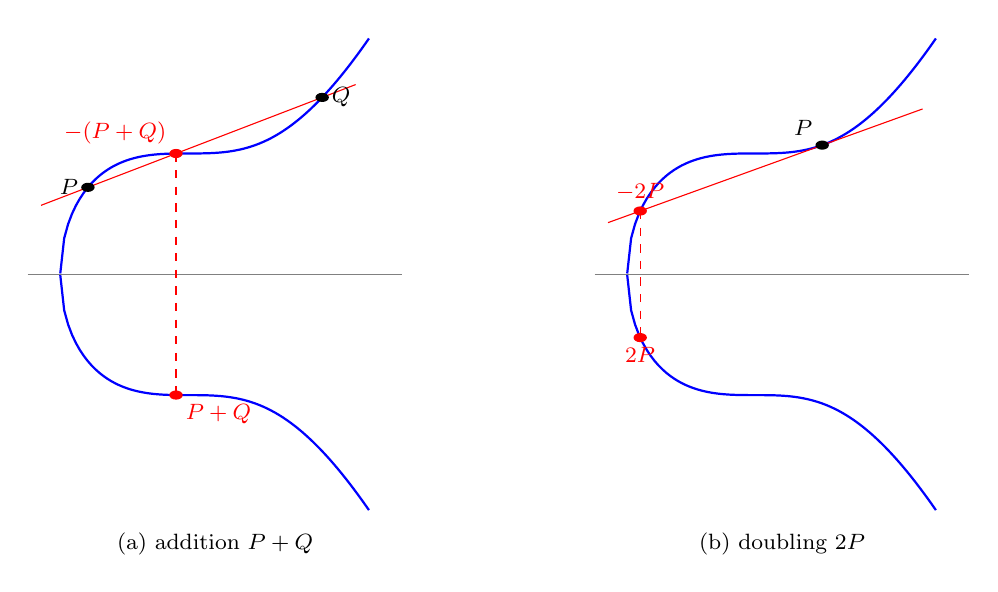
\begin{tikzpicture}[x=0.85cm,y=0.58cm]
\begin{scope}
\clip (-2.4,-5.4) rectangle (3.2,5.4);
\draw[thin,gray] (-2.4,0) -- (3.2,0);
\draw[thick,blue] plot[domain=-1.9129:2.7,samples=80] ({\x},{sqrt(\x*\x*\x+7)});
\draw[thick,blue] plot[domain=-1.9129:2.7,samples=80] ({\x},{-sqrt(\x*\x*\x+7)});
\draw[red] (-2.2,1.51) -- (2.5,4.154);
\draw[dashed,red] (-0.1835,2.6446) -- (-0.1835,-2.6446);
\end{scope}
\fill (-1.5,1.904) circle (0.1) node[left,font=\footnotesize] {$P$};
\fill (2,3.873) circle (0.1) node[right,font=\footnotesize] {$Q$};
\fill[red] (-0.1835,2.6446) circle (0.1) node[above left,font=\footnotesize] {$-(P+Q)$};
\fill[red] (-0.1835,-2.6446) circle (0.1) node[below right,font=\footnotesize] {$P+Q$};
\node[font=\footnotesize] at (0.4,-5.9) {(a) addition $P+Q$};
\begin{scope}[xshift=7.2cm]
\clip (-2.4,-5.4) rectangle (3.2,5.4);
\draw[thin,gray] (-2.4,0) -- (3.2,0);
\draw[thick,blue] plot[domain=-1.9129:2.7,samples=80] ({\x},{sqrt(\x*\x*\x+7)});
\draw[thick,blue] plot[domain=-1.9129:2.7,samples=80] ({\x},{-sqrt(\x*\x*\x+7)});
\draw[red] (-2.2,1.131) -- (2.5,3.62);
\draw[dashed,red] (-1.7188,1.386) -- (-1.7188,-1.386);
\end{scope}
\begin{scope}[xshift=7.2cm]
\fill (1,2.828) circle (0.1) node[above left,font=\footnotesize] {$P$};
\fill[red] (-1.7188,1.386) circle (0.1) node[above,font=\footnotesize] {$-2P$};
\fill[red] (-1.7188,-1.386) circle (0.1) node[below,font=\footnotesize] {$2P$};
\node[font=\footnotesize] at (0.4,-5.9) {(b) doubling $2P$};
\end{scope}
\end{tikzpicture}
\caption{Point addition and doubling on the curve $y^2=x^3+7$ over the real numbers. In (a) the line through $P$ and $Q$ meets the curve in a third point, whose mirror image is $P+Q$. In (b) the tangent at $P$ plays the role of the line.}\label{fig:ecgeom}
\end{figure}

Over a finite field the curve is a scattered set of points and the pictures no longer apply, but the same operation is given by formulas, which are derived from the geometric construction.

\begin{definition}[Point addition and doubling]
Let $P=(x_1,y_1)$ and $Q=(x_2,y_2)$ be points on $E$ with $Q\ne -P$. Then $P+Q=(x_3,y_3)$ with
\[
x_3=s^2-x_1-x_2 \bmod p,\qquad y_3=s(x_1-x_3)-y_1 \bmod p,
\]
where the slope $s$ is
\[
s=\begin{cases}\dfrac{y_2-y_1}{x_2-x_1} \bmod p & \text{if } P\ne Q\quad(\text{point addition}),\\[2ex] \dfrac{3x_1^2+a}{2y_1} \bmod p & \text{if } P=Q\quad(\text{point doubling}).\end{cases}
\]
For $Q=-P$ the result is $P+Q=\mathcal{O}$. For $\mathcal{O}$ the rule is $P+\mathcal{O}=\mathcal{O}+P=P$.
\end{definition}

For our curves $a=0$, so the doubling slope is $3x_1^2/(2y_1)$. The division in the slope means multiplying by a modular inverse.

\begin{theorem}
The points of an elliptic curve together with the addition above form an abelian group: the sum of two points is a point of the curve, the addition is associative and commutative, $\mathcal{O}$ is the neutral element, and every point $P=(x,y)$ has the inverse $-P=(x,-y \bmod p)$.
\end{theorem}

The only hard part of the proof is associativity, which is a tedious algebraic computation and is omitted. Because the group is written additively, repeated addition is written as a multiple: $kP=P+P+\dots+P$ ($k$ terms).

\begin{example}[Adding points on a toy curve]\label{ex:ecadd}
Take $p=43$ and the curve $y^2\equiv x^3+7 \pmod{43}$. The condition $4a^3+27b^2=1323\equiv 33\not\equiv 0$ holds. The point $G=(2,12)$ lies on the curve, since $12^2=144\equiv 15$ and $2^3+7=15$.

\emph{Inverse.} The inverse of $G$ is $-G=(2,-12 \bmod 43)=(2,31)$. Indeed $31^2=961\equiv 15$. Adding the two gives $G+(-G)=\mathcal{O}$ because their $x$-coordinates agree and their $y$-coordinates add up to $43\equiv 0$.

\emph{Doubling.} To compute $2G$ the slope is $s=3\cdot 2^2/(2\cdot 12)=12/24$. Since $24\cdot 9=216\equiv 1 \pmod{43}$ we have $24^{-1}=9$ and $s=12\cdot 9=108\equiv 22$. Then $x_3=22^2-2-2=480\equiv 7$ and $y_3=22\,(2-7)-12=-122\equiv 7$, so $2G=(7,7)$. A check: $7^2=49\equiv 6$ and $7^3+7=350\equiv 6$.

\emph{Addition.} To compute $3G=2G+G$ the slope is $s=(12-7)/(2-7)=5/(-5)=-1\equiv 42$. Then $x_3=1-7-2=-8\equiv 35$ and $y_3=-1\cdot(7-35)-7=21$, so $3G=(35,21)$.
\end{example}

\subsection{The number of points and cyclic subgroups}

The security of an elliptic curve system depends on the size of the group, so it is important to know how many points a curve has. The following theorem gives a tight range.

\begin{theorem}[Hasse]
The number of points $\#E$ on an elliptic curve over $\F_p$ satisfies
\[
p+1-2\sqrt p\ \le\ \#E\ \le\ p+1+2\sqrt p .
\]
\end{theorem}

In words, the number of points is close to $p$, so a curve over a $256$-bit prime has about $2^{256}$ points, and the group is about as large as the field.

The \emph{order} of a point $P$ is the smallest $k>0$ with $kP=\mathcal{O}$. The order of every point divides $\#E$, so if $\#E$ is a prime then every point other than $\mathcal{O}$ has order $\#E$ and generates the whole group. Such a point is called a primitive element or generator. The curve \texttt{secp256k1} has this property: its number of points is a prime $n\approx 2^{256}$, and Bitcoin fixes one generator $G$ for everybody.

\begin{example}[The toy curve and its multiples]\label{ex:curve}
The curve $y^2\equiv x^3+7$ over $\F_{43}$ has $30$ points with coordinates, so with $\mathcal{O}$ the group has $\#E=31$ elements. This agrees with Hasse's theorem, which for $p=43$ allows $44-2\sqrt{43}\approx 30.9$ up to $44+2\sqrt{43}\approx 57.1$ points. Since $31$ is a prime, every point other than $\mathcal{O}$ generates the whole group, and we use $G=(2,12)$. From now on $n=31$. Repeated addition produces all multiples of $G$:
\begin{center}\small
\begin{tabular}{rl@{\qquad}rl@{\qquad}rl}
\toprule
$k$ & $kG$ & $k$ & $kG$ & $k$ & $kG$\\
\midrule
1 & (2,12) & 11 & (40,25) & 21 & (42,36)\\
2 & (7,7) & 12 & (37,36) & 22 & (20,3)\\
3 & (35,21) & 13 & (13,21) & 23 & (32,3)\\
4 & (21,18) & 14 & (34,40) & 24 & (25,25)\\
5 & (12,12) & 15 & (38,21) & 25 & (29,12)\\
6 & (29,31) & 16 & (38,22) & 26 & (12,31)\\
7 & (25,18) & 17 & (34,3) & 27 & (21,25)\\
8 & (32,40) & 18 & (13,22) & 28 & (35,22)\\
9 & (20,40) & 19 & (37,7) & 29 & (7,36)\\
10 & (42,7) & 20 & (40,18) & 30 & (2,31)\\
\bottomrule
\end{tabular}
\end{center}
The next multiple is $31G=\mathcal{O}$, after which the list repeats. The multiples $kG$ and $(31-k)G$ have the same $x$-coordinate and opposite $y$-coordinates, since $(31-k)G=-kG$.
\end{example}

\subsection{The elliptic curve discrete logarithm problem}

\begin{definition}[Elliptic curve discrete logarithm problem (ECDLP)]
Let $E$ be an elliptic curve and $G$ a point of prime order $n$. Given a point $Q=dG$ in the subgroup generated by $G$, find the integer $d$ with $1\le d\le n-1$.
\end{definition}

The integer $d$ is the secret key, and the point $Q=dG$ is the public key. On the toy curve one finds $d$ by looking $Q$ up in the table of Example~\ref{ex:curve}. On \texttt{secp256k1} the table would have $2^{256}$ rows.

Computing $Q=dG$ for a known $d$ does not require $d$ additions. The \emph{double-and-add} algorithm scans the bits of $d$ from the most significant bit down: for each further bit it doubles the current point, and if the bit is $1$ it also adds $G$. This takes at most $2\log_2 d$ group operations, which is about $512$ operations for a $256$-bit $d$.

\begin{example}[Double-and-add]\label{ex:dbl}
To compute $13G$ on the toy curve, write $13=1101_2$. Start with the leading bit: $G$. The next bit is $1$: double and add, $2G+G=3G$. The next bit is $0$: double only, $2\cdot 3G=6G$. The last bit is $1$: double and add, $2\cdot 6G+G=12G+G=13G$. Four bits gave three doublings and two additions. The result agrees with the table, $13G=(13,21)$.
\end{example}

The best known attacks on the ECDLP for well-chosen curves are generic ones such as Pollard's rho method, which needs about $\sqrt n$ group operations. A curve with a $256$-bit order therefore offers $128$ bits of security. Table~\ref{tab:keysizes} compares the sizes of curves and RSA moduli that offer the same security level.

\begin{table}[h]
\centering
\begin{tabular}{rrr}
\toprule
Security level (bits) & Elliptic curve (bits) & RSA modulus (bits)\\
\midrule
80 & 160 & 1024\\
112 & 224 & 2048\\
128 & 256 & 3072\\
192 & 384 & 7680\\
256 & 512 & 15360\\
\bottomrule
\end{tabular}
\caption{Bit lengths that give comparable classical security. Bitcoin's curve has a $256$-bit group order and therefore provides about $128$ bits of security.}\label{tab:keysizes}
\end{table}

\subsection{Diffie--Hellman key exchange on elliptic curves}

The discrete logarithm problem allows two parties to agree on a secret over an open channel. The elliptic curve version works as follows. Alice and Bob agree on a curve $E$ and a generator $G$ of order $n$. Alice picks a secret $a$ and sends $A=aG$. Bob picks a secret $b$ and sends $B=bG$. Alice computes $S=aB$ and Bob computes $S=bA$. Both obtain the same point, because $aB=a(bG)=(ab)G=b(aG)=bA$. An eavesdropper sees $A$ and $B$ and would need $a$ or $b$, which means solving the ECDLP.

\begin{figure}[h]
\centering
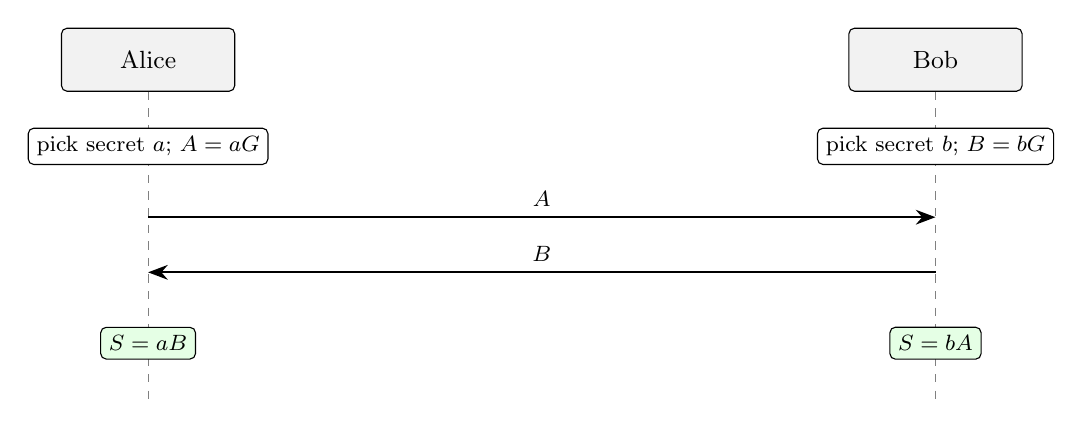
\begin{tikzpicture}[x=1cm,y=1cm]
\node[actor] (A) at (0,0) {Alice};
\node[actor] (B) at (10,0) {Bob};
\draw[life] (A) -- (0,-4.4); \draw[life] (B) -- (10,-4.4);
\node[box] at (0,-1.1) {pick secret $a$;\ $A=aG$};
\node[box] at (10,-1.1) {pick secret $b$;\ $B=bG$};
\draw[msg] (0,-2.0) -- (10,-2.0) node[midway,above,font=\footnotesize] {$A$};
\draw[msg] (10,-2.7) -- (0,-2.7) node[midway,above,font=\footnotesize] {$B$};
\node[box,fill=green!10] at (0,-3.6) {$S=aB$};
\node[box,fill=green!10] at (10,-3.6) {$S=bA$};
\end{tikzpicture}
\caption{Elliptic curve Diffie--Hellman. Both parties end up with the same point $S=abG$, and only $A$ and $B$ cross the open channel.}
\end{figure}

\begin{example}[Key exchange on the toy curve]\label{ex:ecdh}
Alice picks $a=4$ and sends $A=4G=(21,18)$. Bob picks $b=9$ and sends $B=9G=(20,40)$. Alice computes $S=aB=4\cdot 9G=36G=5G=(12,12)$, using $36=31+5$. Bob computes $S=bA=9\cdot 4G=36G=(12,12)$. Both hold the shared point $(12,12)$, and a symmetric key can be derived from it, for instance by hashing its $x$-coordinate.
\end{example}

Diffie--Hellman by itself does not authenticate anybody, since it gives no way of telling whom one is talking to. Signatures solve this, and the two are combined in Section~\ref{sec:tls}.


\subsection{Schnorr signatures}\label{sec:schnorr}

Schnorr signatures are easiest to understand as the result of a short interactive protocol in which Alice proves that she knows $d$, followed by a trick that removes the interaction.

\emph{The interactive proof.} Alice's key pair is $(d,Q)$ with $Q=dG$. To prove knowledge of $d$ without revealing it, she picks a fresh random number $k$ and sends the commitment $R=kG$. Bob answers with a random challenge $e$. Alice responds with $s=k+ed \bmod n$. Bob checks whether $sG = R + eQ$. This holds for an honest Alice because $sG=(k+ed)G=kG+e\,(dG)=R+eQ$. The number $k$ hides $d$ in the response: without $k$, the value $s$ is just a random-looking number modulo $n$.

\begin{figure}[h]
\centering
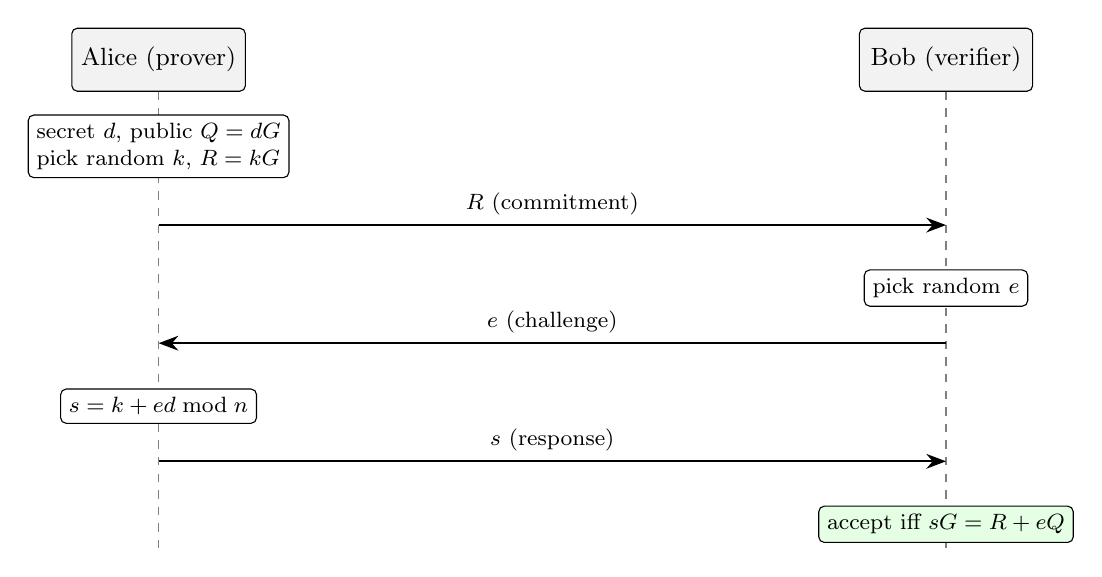
\begin{tikzpicture}[x=1cm,y=1cm]
\node[actor] (A) at (0,0) {Alice (prover)};
\node[actor] (B) at (10,0) {Bob (verifier)};
\draw[life] (A) -- (0,-6.2); \draw[life] (B) -- (10,-6.2);
\node[box,align=left] at (0,-1.1) {secret $d$, public $Q=dG$\\pick random $k$, $R=kG$};
\draw[msg] (0,-2.1) -- (10,-2.1) node[midway,above,font=\footnotesize] {$R$ (commitment)};
\node[box] at (10,-2.9) {pick random $e$};
\draw[msg] (10,-3.6) -- (0,-3.6) node[midway,above,font=\footnotesize] {$e$ (challenge)};
\node[box] at (0,-4.4) {$s=k+ed \bmod n$};
\draw[msg] (0,-5.1) -- (10,-5.1) node[midway,above,font=\footnotesize] {$s$ (response)};
\node[box,fill=green!10] at (10,-5.9) {accept iff $sG=R+eQ$};
\end{tikzpicture}
\caption{The Schnorr identification protocol. Making Bob's challenge $e$ the output of a hash function, $e=\Hash(R\Vert Q\Vert m)$, turns this protocol into a signature on $m$.}
\end{figure}

\emph{From proof to signature.} Alice would like to prove her knowledge of $d$ without Bob being online. She replaces Bob's random challenge by a hash that she cannot control: $e=\Hash(R\Vert Q\Vert m)$. The message $m$ is included in the hash, so the proof is tied to $m$. Anybody can recompute $e$, so anybody can verify. This transformation is called the Fiat--Shamir transform, and Section~3 uses it again for lattices.

\begin{definition}[Schnorr signature]
\emph{Keys.} $\sk=d\in\{1,\dots,n-1\}$, $\pk=Q=dG$.

\emph{Signing.} Choose a fresh random $k\in\{1,\dots,n-1\}$ and compute $R=kG$, $e=\Hash(R\Vert Q\Vert m) \bmod n$ and $s=k+ed \bmod n$. The signature is $(R,s)$.

\emph{Verification.} Compute $e=\Hash(R\Vert Q\Vert m) \bmod n$ and accept iff $sG=R+eQ$.
\end{definition}

\begin{example}[Schnorr signing and verification]\label{ex:schnorr}
On the curve of Example~\ref{ex:curve}, Alice chooses the secret key $d=7$. Her public key is $Q=7G=(25,18)$, read from the table. To sign a message she chooses $k=10$ and computes $R=10G=(42,7)$. Suppose the (toy) hash value is $e=\Hash(R\Vert Q\Vert m) \bmod 31=13$. Then
\[
s=k+ed=10+13\cdot 7=101\equiv 8 \pmod{31},
\]
and the signature is $\big(R,s\big)=\big((42,7),\,8\big)$.

Bob recomputes $e=13$ and checks both sides of $sG=R+eQ$. The left side is $8G=(32,40)$. For the right side he first needs $eQ=13Q=13\cdot 7G=91G=29G=(7,36)$, because $91=2\cdot 31+29$. Adding $R=(42,7)$ and $(7,36)$ uses the slope $\lambda=(36-7)/(7-42)=29/(-35)=29/8$. Since $8^{-1}=27$ modulo $43$, $\lambda=29\cdot 27=783\equiv 9$. Then $x_3=81-42-7=32$ and $y_3=9(42-32)-7=83\equiv 40$, so $R+eQ=(32,40)$. Both sides agree and Bob accepts.
\end{example}

\emph{Why $k$ must be fresh and secret.} If Eve learns $k$, then $d=(s-k)\,e^{-1}$ follows by one modular computation. In the example, $d=(8-10)\cdot 13^{-1} \bmod 31$; since $13\cdot 12=156\equiv 1$ we get $13^{-1}=12$ and $d=(-2)\cdot 12=-24\equiv 7$.

\subsection{ECDSA}

ECDSA is the older and more intricate sibling. It does not hash the nonce point into the challenge and it uses a modular inverse in the signing equation.

\begin{definition}[ECDSA]
\emph{Keys.} $\sk=d\in\{1,\dots,n-1\}$, $\pk=Q=dG$.

\emph{Signing.} Let $z=\Hash(m)$, reduced to an integer modulo $n$. Choose a fresh random $k\in\{1,\dots,n-1\}$ and compute $R=kG=(x_R,y_R)$ and $r=x_R \bmod n$. Compute $s=k^{-1}(z+rd) \bmod n$. If $r=0$ or $s=0$ choose a new $k$. The signature is $(r,s)$.

\emph{Verification.} Check that $r,s\in\{1,\dots,n-1\}$. Compute $w=s^{-1} \bmod n$, $u_1=zw \bmod n$, $u_2=rw \bmod n$ and $P=u_1G+u_2Q$. Accept iff $P\ne\mathcal{O}$ and $x_P \bmod n=r$.
\end{definition}

\begin{theorem}[Correctness]
For an honest signature, $P=kG$.
\end{theorem}
\begin{proof}
From $s=k^{-1}(z+rd)$ we get $k=s^{-1}(z+rd)=zw+rwd=u_1+u_2d \pmod n$. Hence $P=u_1G+u_2Q=(u_1+u_2d)G=kG=R$, and so $x_P \bmod n=r$.
\end{proof}

\begin{example}[ECDSA signing and verification]\label{ex:ecdsa}
Use the same keys, $d=7$ and $Q=(25,18)$. Suppose the hash of the message reduces to $z=20$. Alice chooses $k=10$ and computes $R=10G=(42,7)$, so $r=42 \bmod 31=11$. Her signature value is
\[
s = 10^{-1}(z+rd) = 10^{-1}(20+11\cdot 7) = 10^{-1}\cdot 97 \bmod 31.
\]
Since $10\cdot 28=280\equiv 1 \pmod{31}$ we have $10^{-1}=28$, and $97\equiv 4$, so $s=4\cdot 28=112\equiv 19$. The signature is $(r,s)=(11,19)$.

Bob computes $w=19^{-1}=18$ (since $19\cdot 18=342=11\cdot 31+1$), $u_1=20\cdot 18=360\equiv 19$ and $u_2=11\cdot 18=198\equiv 12$. Then
\[
P=19G+12Q=19G+12\cdot 7G=19G+84G=19G+22G=41G=10G=(42,7),
\]
using $84=2\cdot 31+22$ and $41=31+10$. Its $x$-coordinate is $42$ and $42 \bmod 31=11=r$, so Bob accepts.
\end{example}

\begin{remark}[Schnorr versus ECDSA]
Schnorr's equation $s=k+ed$ is linear in the secret values, which makes it easy to prove secure and allows signatures and keys to be added together (see the end of this section). ECDSA's equation has $k^{-1}$ in it, which destroys linearity, and its verification needs a modular inverse and two scalar multiplications. ECDSA signatures are also malleable: if $(r,s)$ is valid then so is $(r,n-s)$. In the example, $(11,12)$ is also accepted, since $12^{-1}=13$, $u_1=12$, $u_2=19$ and $12G+19\cdot 7G=21G=(42,36)$, which has the same $x$-coordinate $42$. Bitcoin therefore requires the ``low-$s$'' form to stop third parties from changing a transaction's identifier.
\end{remark}

\subsection{Nonce reuse: why the nonce must never repeat}

A signature reveals one linear equation in two unknowns, $d$ and $k$. A second signature with the same $k$ gives a second equation, and then both unknowns can be solved.

\begin{example}[Recovering the secret key from a repeated nonce]\label{ex:nonce}
Alice signs two different messages with $z_1=20$ and $z_2=9$ but, through a faulty random number generator, uses $k=10$ both times. Both signatures have the same $r=11$, which is visible to everybody. The $s$-values are $s_1=19$ (from the previous example) and $s_2=10^{-1}(9+77)=28\cdot 86 \equiv 28\cdot 24=672\equiv 21 \pmod{31}$.

Eve subtracts the two equations $s_1k=z_1+rd$ and $s_2k=z_2+rd$ and gets $(s_1-s_2)k=z_1-z_2$, so
\[
k=\frac{z_1-z_2}{s_1-s_2}=\frac{11}{-2}\equiv 11\cdot 15=165\equiv 10 \pmod{31},
\]
because $(-2)^{-1}=29^{-1}=15$. With $k$ known, $d=(s_1k-z_1)\,r^{-1}=(190-20)\cdot 17=170\cdot 17\equiv 15\cdot 17=255\equiv 7 \pmod{31}$, since $11^{-1}=17$. Eve has recovered $d=7$ and can now sign anything as Alice.
\end{example}

This is not a theoretical danger. In 2010 the signing key of the Sony PlayStation 3 was recovered because Sony used a constant $k$, and in 2013 several Android Bitcoin wallets lost coins because their random number generator repeated nonces. Modern implementations derive $k$ deterministically from $(d,z)$ (RFC~6979 for ECDSA and the nonce derivation in BIP~340 for Schnorr), so that two different messages never share a nonce.

\subsection{Signatures in a Bitcoin transaction}

A Bitcoin coin is not a file but an unspent transaction output, which is locked with a condition. In the most common case the condition is ``whoever shows a public key whose hash equals $X$ together with a valid signature for it may spend this output.'' The value $X$ is the hash of the owner's public key, and it is what an address encodes.

Alice has an output locked to her key and wants to pay Bob. She builds a new transaction that names the old output as input and lists the new outputs: an amount for Bob's address, the change returning to herself, and the fee. She hashes the transaction data $z=\Hash(\text{tx})$ and signs $z$ with her secret key $d$. The signature and the public key $Q$ are attached to the input. Every node on the network then checks three things: that $\Hash(Q)$ equals the value in the lock, that the signature is valid for $Q$ and $z$, and that the old output was not spent before.

\begin{figure}[h]
\centering
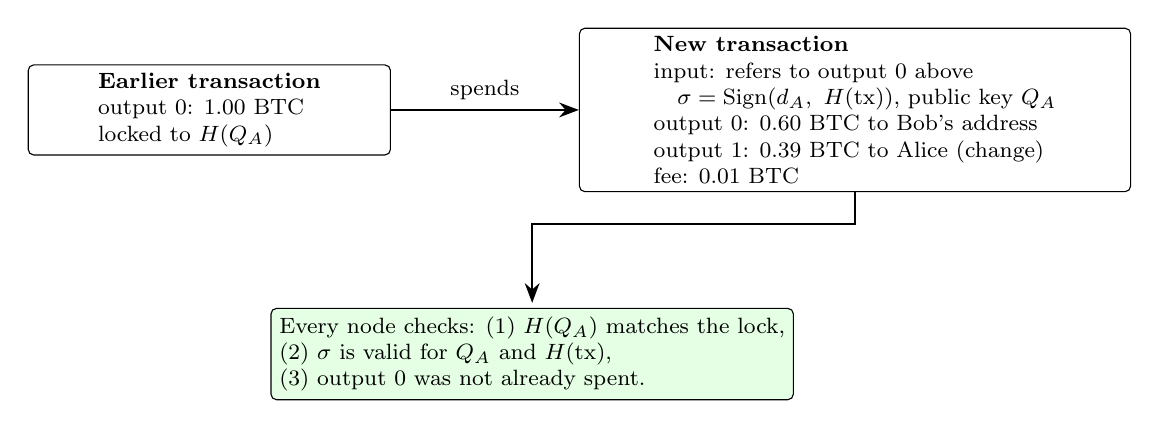
\begin{tikzpicture}[x=1cm,y=1cm]
\node[box,align=left,minimum width=4.6cm] (old) at (0,0) {\textbf{Earlier transaction}\\output 0: 1.00 BTC\\locked to $\Hash(Q_A)$};
\node[box,align=left,minimum width=7cm] (new) at (8.2,0) {\textbf{New transaction}\\input: refers to output 0 above\\\quad $\sigma=\mathrm{Sign}(d_A,\ \Hash(\text{tx}))$,\ public key $Q_A$\\output 0: 0.60 BTC to Bob's address\\output 1: 0.39 BTC to Alice (change)\\fee: 0.01 BTC};
\draw[msg] (old) -- (new) node[midway,above,font=\footnotesize] {spends};
\node[box,fill=green!10,align=left] at (4.1,-3.1) {Every node checks: (1) $\Hash(Q_A)$ matches the lock,\\(2) $\sigma$ is valid for $Q_A$ and $\Hash(\text{tx})$,\\(3) output 0 was not already spent.};
\draw[msg] (new.south) -- ++(0,-0.4) -| (4.1,-2.45);
\end{tikzpicture}
\caption{Spending a coin. With the default signature hash type the signature covers all outputs, so changing the amount or Bob's address after signing makes the signature invalid.}
\end{figure}

\begin{example}[Why Oscar cannot redirect the payment]
Alice's transaction sends $0.60$ BTC to Bob's address. Oscar sees the transaction in the network before it is confirmed and replaces Bob's address with his own. The transaction data changes, so its hash changes from $z$ to $z'$. Alice's signature $(r,s)$ was computed for $z$. For $z'$ the verification equation yields a point $P'=u_1'G+u_2Q$ whose $x$-coordinate no longer equals $r$, except with negligible probability. The nodes reject Oscar's version, and he cannot sign $z'$ himself since he does not know $d$.
\end{example}

\subsection{Linearity of Schnorr: adding signatures}

The linear equation $s=k+ed$ has a useful consequence. If Alice and Bob each hold a secret key and want a single signature for the joint key $Q=Q_A+Q_B$, each of them signs with the sum of the nonces and the sum of the signatures is again a valid signature. This is the idea behind multi-signatures such as MuSig and is one reason Bitcoin adopted Schnorr.

\begin{example}[Two signers, one signature]\label{ex:musig}
Let Alice use $d_A=7$ and Bob use $d_B=5$, so $Q_A=7G=(25,18)$ and $Q_B=5G=(12,12)$. The joint key is $Q=Q_A+Q_B=12G=(37,36)$. They choose nonces $k_A=10$ and $k_B=3$ and exchange $R_A=10G$ and $R_B=3G$, so the joint nonce point is $R=R_A+R_B=13G=(13,21)$. The challenge is $e=\Hash(R\Vert Q\Vert m)=13$ (toy value). Each partner computes a partial response,
\[
s_A=k_A+ed_A=10+91=101\equiv 8,\qquad s_B=k_B+ed_B=3+65=68\equiv 6 \pmod{31},
\]
and the sum is $s=s_A+s_B=14$. The pair $(R,s)$ is an ordinary Schnorr signature for $Q$: $sG=14G=(34,40)$ and $R+eQ=13G+13\cdot 12G=13G+156G=169G=14G$, since $169=5\cdot 31+14$. The verifier cannot tell that two people signed. (This simple key addition is vulnerable to a rogue-key attack in which one partner chooses a key depending on the other's. MuSig2 defends against it by weighting each key with a hash-derived coefficient.)
\end{example}

%=====================================================================
\section{Lattice-Based Signatures}
%=====================================================================

\subsection{Why lattices, and the names involved}

RSA, ECDSA and Schnorr all fall to Shor's algorithm on a large quantum computer, since it solves both factoring and discrete logarithms in polynomial time. Lattice problems have no known quantum speed-up of this kind. Two design ideas dominate lattice signatures, and each has its own pair of names attached.

The first is \emph{hash-and-sign}. It was proposed by Goldreich, Goldwasser and Halevi (the GGH signature, 1997), followed by NTRUSign of Hoffstein, Pipher and Silverman (2003). Both were broken by Nguyen and Regev (2006), who showed that the signatures leak the secret basis (see below). Gentry, Peikert and Vaikuntanathan (2008) repaired the idea with Gaussian sampling, and Falcon (named FN-DSA in the draft NIST standard FIPS~206) is a refined version of this repair on NTRU lattices.

The second is the \emph{Fiat--Shamir} approach. Fiat and Shamir (1986) showed how to turn an interactive identification protocol into a signature, which Section~2 used for Schnorr. Lyubashevsky (2009) made this work for lattices with a technique called \emph{rejection sampling} (``Fiat--Shamir with aborts''). CRYSTALS-Dilithium is built on it and has been standardized by NIST as ML-DSA (FIPS~204). Because the transform is due to Fiat and Shamir, this family is called Fiat--Shamir lattice signatures.

Section~3.3 explains hash-and-sign through a picture in two dimensions. Section~3.4 explains Fiat--Shamir with aborts through a full numerical example.

\subsection{Lattice background}

A lattice is the set of all integer combinations of linearly independent basis vectors. With the basis vectors as the rows of a matrix $B$,
\[
\mathcal{L}(B)=\{\,xB : x\in\Z^n\,\}.
\]
The same lattice has many bases: if $U$ is an integer matrix with determinant $\pm 1$, then $UB$ generates the same lattice. A basis with short, nearly orthogonal vectors is \emph{good}, and one with long, skewed vectors is \emph{bad}. Given a target point $h$ that is not on the lattice, the \emph{closest vector problem (CVP)} asks for the lattice point nearest to $h$. A good basis makes CVP easy through Babai's rounding: write $h=cB$ with real coordinates $c$, round $c$ to the nearest integers and output $\lfloor c\rceil B$. A bad basis makes the same rounding land far from $h$.

The second family of hard problems is of a different flavour. Fix a modulus $q$ and a random matrix $A\in\Z_q^{n\times m}$. The \emph{short integer solution problem (SIS)} asks for a nonzero short $z\in\Z^m$ with $Az\equiv 0 \pmod q$. The \emph{learning with errors problem (LWE)} asks to recover a short $s_1$ from $(A,\,t=As_1+s_2 \bmod q)$ where $s_2$ is a short error vector, and it is believed that $t$ is indistinguishable from random. Both have security reductions from worst-case lattice problems. Fiat--Shamir lattice signatures use LWE for the key and SIS for unforgeability.

\subsection{Hash-and-sign: GGH in two dimensions}

The idea is a trapdoor built from the difference between good and bad bases. Alice generates a lattice together with a good basis $G$ and publishes a bad basis $B$ of the same lattice. Signing a message means finding a lattice point close to the hash of the message, which is a CVP instance that only the owner of the good basis can solve. Verifying means checking that the point is on the lattice and close, which anybody can do with any basis.

\begin{definition}[GGH-style signature]
\emph{Keys.} $\sk=G$ (good basis), $\pk=B=UG$ with $U$ a unimodular matrix that makes $B$ bad.

\emph{Signing.} Map $m$ to a target point $h=\Hash(m)\in\Z^n$. Compute $v=\lfloor hG^{-1}\rceil\,G$ with Babai rounding and output $\sigma=v$.

\emph{Verification.} Accept iff $vB^{-1}$ has integer entries (so $v\in\mathcal{L}(B)$) and $\norm{v-h}\le\rho$, where the bound $\rho$ is chosen so that honest signatures always pass.
\end{definition}

\begin{example}[Key generation in dimension two]\label{ex:ggh-key}
Let the good basis be $b_1=(6,1)$ and $b_2=(-1,6)$. These two vectors have length $\sqrt{37}\approx 6.08$ and are orthogonal, and they span a lattice of determinant $37$. Choose the unimodular matrix $U=\begin{pmatrix}2&5\\5&13\end{pmatrix}$, which has determinant $26-25=1$. The public basis is
\[
b_1'=2b_1+5b_2=(7,32),\qquad b_2'=5b_1+13b_2=(17,83).
\]
Both vectors generate the same lattice as $b_1,b_2$ but are much longer and nearly parallel. For Babai rounding in two dimensions the error is at most $\tfrac12(\norm{b_1}+\norm{b_2})=\sqrt{37}\approx 6.08$, so we set $\rho=6.1$.
\end{example}

\begin{example}[Signing and verifying]\label{ex:ggh-sign}
Suppose the message hashes to the point $h=(20,25)$.

\emph{Alice signs with the good basis.} Writing $h=cG$ gives $c=hG^{-1}=\tfrac1{37}(145,\,130)\approx(3.92,\,3.51)$. Rounding gives $(4,4)$, so
\[
v=4b_1+4b_2=(24-4,\ 4+24)=(20,28),\qquad \norm{v-h}=\norm{(0,3)}=3\le 6.1.
\]
The signature is $v=(20,28)$.

\emph{Bob verifies with the public basis.} He computes $vB^{-1}=\tfrac1{37}(20\cdot 83-28\cdot 17,\ -20\cdot 32+28\cdot 7)=\tfrac1{37}(1184,\,-444)=(32,\,-12)$. These are integers, so $v=32b_1'-12b_2'$ is on the lattice, and $\norm{v-h}=3\le\rho$, so he accepts.

\emph{Eve tries with the bad basis.} Eve knows only $b_1',b_2'$. Babai rounding with these gives the coordinates $hB^{-1}=\tfrac1{37}(1235,\,-465)\approx(33.4,\,-12.6)$, which round to $(33,-13)$ and the lattice point $33b_1'-13b_2'=(10,-23)$. This point is on the lattice but at distance $\norm{(10,-23)-(20,25)}\approx 49$ from $h$, far above the bound $\rho=6.1$, so it is rejected.
\end{example}

\begin{figure}[h]
\centering
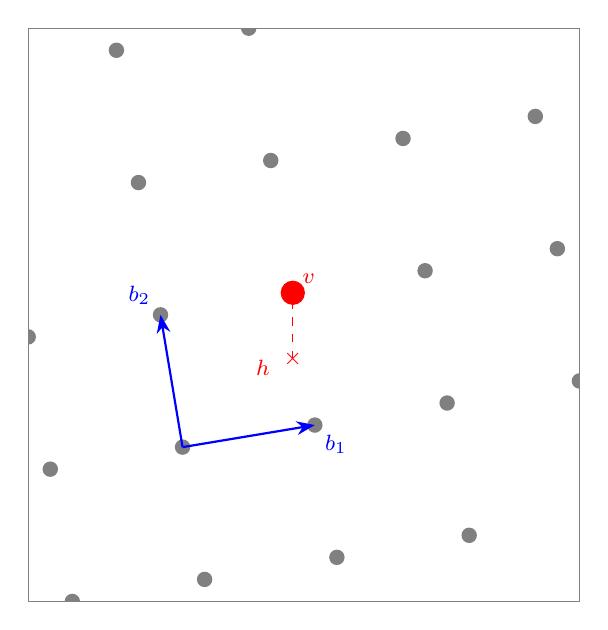
\begin{tikzpicture}[x=0.28cm,y=0.28cm]
\begin{scope}
\clip (8,14) rectangle (33,40);
\foreach \i in {0,...,9}{\foreach \j in {0,...,9}{
  \pgfmathsetmacro\px{6*\i-\j}\pgfmathsetmacro\py{\i+6*\j}
  \fill[gray] (\px,\py) circle (0.35);}}
\end{scope}
\draw[gray] (8,14) rectangle (33,40);
\draw[-{Stealth},thick,blue] (15,21) -- (21,22) node[below right,font=\footnotesize] {$b_1$};
\draw[-{Stealth},thick,blue] (15,21) -- (14,27) node[above left,font=\footnotesize] {$b_2$};
\draw[dashed,red] (20,25) -- (20,28);
\node[red,font=\footnotesize] at (20,25) {$\times$};
\node[red,font=\footnotesize,left] at (19.4,24.6) {$h$};
\fill[red] (20,28) circle (0.55);
\node[red,font=\footnotesize,above right] at (20,28) {$v$};
\end{tikzpicture}
\caption{A window of the lattice generated by $b_1=(6,1)$ and $b_2=(-1,6)$ (grey points). The target $h=(20,25)$ is marked $\times$ and the lattice point $v=4b_1+4b_2=(20,28)$ is the signature. The public bad basis $(7,32),(17,83)$ describes the same grey points but its vectors are far too long to appear in this window.}
\end{figure}

\emph{Why the plain version is broken.} Every signature gives the signer's error vector $v-h$, and by construction this vector lies in the parallelepiped $\{a b_1+b\,b_2:\ |a|,|b|\le\tfrac12\}$ spanned by the secret basis. In the example the two errors observed so far are $(0,3)$ for $h=(20,25)$ and $(2,-2)$ for a second target $h_2=(-13,31)$ (whose Babai point is $(-11,29)$). Both have coordinates in $[-\tfrac12,\tfrac12]$ with respect to $G$: $(0,3)G^{-1}=\tfrac1{37}(3,18)$ and $(2,-2)G^{-1}=\tfrac1{37}(10,-14)$. With enough signatures the errors fill the whole parallelepiped, and its edges are the secret basis vectors. Nguyen and Regev (2006) turned this observation into an efficient attack, called learning a parallelepiped, and it broke GGH and NTRUSign.

\emph{The repair.} Gentry, Peikert and Vaikuntanathan make the signature leak nothing by choosing $v$ at random from a discrete Gaussian distribution on the lattice centred at $h$, using the good basis only as a sampling tool. The error $v-h$ then follows the same Gaussian distribution whatever the secret basis is, so signatures carry no information about it. Falcon implements this idea efficiently on NTRU lattices.

\subsection{Fiat--Shamir with aborts}

The second family avoids good and bad bases altogether and follows the Schnorr design of Section~\ref{sec:schnorr}: commit, challenge, respond. The lattice version is built from the following public-key structure.

\emph{Keys.} Let $A$ be a public random matrix modulo $q$. The secret key is a pair of short vectors $(s_1,s_2)$ and the public key is $t=As_1+s_2 \bmod q$. Recovering $(s_1,s_2)$ from $(A,t)$ is an LWE problem.

\emph{Commit, challenge, respond.} To sign $m$, Alice picks a random masking vector $y$, computes the commitment $w=Ay$, derives a short challenge $c=\Hash(w,m)$ and responds with $z=y+cs_1$. Bob checks that $Az-ct$ reproduces the commitment. The algebra is
\[
Az-ct=A y+cAs_1-c(As_1+s_2)=Ay-cs_2=w-cs_2 .
\]
Two difficulties arise. The first is that Bob obtains $w-cs_2$, not $w$. The difference $cs_2$ is small, so the fix is to hash only the \emph{high-order bits} of $w$. Bob's slightly wrong value then has the same high bits as $w$, except in unlucky cases, and in those cases Alice detects the problem herself and restarts. The second is that $z=y+cs_1$ would leak $s_1$ if $y$ were not hidden well, which the aborts handle.

\begin{definition}[Toy Fiat--Shamir lattice signature]\label{def:toyfs}
Parameters: modulus $q=97$, bound $\gamma=20$ for the masking vector, $\beta=1$ for the size of $cs_1$, and $\HB(x)=\lfloor x/8\rfloor$ for $x\in\{0,\dots,96\}$ applied to each coordinate. Challenges are $c\in\{-1,+1\}$ and the toy hash is $c=+1$ if the sum of the entries of $\HB(w)$ plus the sum of the ASCII codes of $m$ is even, and $c=-1$ otherwise.

\emph{Keys.} $\sk=(s_1,s_2)$ with small entries and $\pk=(A,t)$ with $t=As_1+s_2 \bmod q$.

\emph{Signing.}
\begin{enumerate}[nosep]
\item Choose $y$ with every entry uniform in $\{-\gamma,\dots,\gamma\}$. Compute $w=Ay \bmod q$.
\item Compute $c=\Hash(\HB(w),m)$ and $z=y+cs_1$.
\item If some entry of $z$ has absolute value $>\gamma-\beta$, or if $\HB(w-cs_2)\ne\HB(w)$, abort and start again at step 1.
\item Output $\sigma=(z,c)$.
\end{enumerate}

\emph{Verification.} Compute $w'=Az-ct \bmod q$. Accept iff every entry of $z$ has absolute value $\le\gamma-\beta$ and $c=\Hash(\HB(w'),m)$.
\end{definition}

\begin{example}[Key generation]\label{ex:fs-key}
Let
\[
A=\begin{pmatrix}23&41\\67&12\end{pmatrix},\qquad s_1=\begin{pmatrix}1\\-1\end{pmatrix},\qquad s_2=\begin{pmatrix}0\\1\end{pmatrix}.
\]
Then $As_1=(23-41,\ 67-12)=(-18,55)$, and $t=As_1+s_2=(-18,56)\equiv(79,56) \pmod{97}$. The public key is $(A,t)$ with $t=(79,56)$. Anybody can see $t$, but finding the short vectors $(s_1,s_2)$ behind it is the LWE problem. Here the entries are tiny so that the search is trivial. In ML-DSA the vectors have hundreds of entries over a polynomial ring.
\end{example}

\begin{example}[Signing with aborts]\label{ex:fs-sign}
Alice signs $m=\text{``PAY BOB 100''}$, whose ASCII codes add up to $654$. The bound for $z$ is $\gamma-\beta=19$. Her attempts are:

\begin{center}\footnotesize\setlength{\tabcolsep}{3pt}
\begin{tabular}{clllllll}
\toprule
\# & $y$ & $w=Ay \bmod 97$ & $\HB(w)$ & $c$ & $z=y+cs_1$ & $\HB(w-cs_2)$ & result\\
\midrule
1 & $(19,-4)$ & $(79,61)$ & $(9,7)$ & $+1$ & $(20,-5)$ & $(9,7)$ & abort: $|20|>19$\\
2 & $(2,13)$ & $(94,96)$ & $(11,12)$ & $-1$ & $(1,14)$ & $(11,0)$ & abort: high bits\\
3 & $(-19,9)$ & $(29,96)$ & $(3,12)$ & $-1$ & $(-20,10)$ & $(3,0)$ & abort: $|-20|>19$\\
4 & $(-5,-17)$ & $(61,43)$ & $(7,5)$ & $+1$ & $(-4,-18)$ & $(7,5)$ & \textbf{accept}\\
\bottomrule
\end{tabular}
\end{center}

The details of attempt~1 are $w=Ay=(23\cdot 19-41\cdot 4,\ 67\cdot 19-12\cdot 4)=(273,\,1225)\equiv(79,61)$, $\HB(w)=(9,7)$, and $9+7+654=670$ is even so $c=+1$. The response $z=y+s_1=(20,-5)$ is too large, so Alice discards the attempt. Attempt~2 passes the size test, but $w-cs_2=(94,96)+(0,1)=(94,97)\equiv(94,0)$ has high bits $(11,0)\ne(11,12)$: adding $1$ wraps the second coordinate from $96$ around to $0$ modulo $97$, so the high bits change and a verifier computing $w-cs_2$ would hash different input. Attempt~4 passes both tests. With $w=(61,43)$, $c=+1$ (since $7+5+654=666$ is even) and $z=y+s_1=(-4,-18)$, the signature is
\[
\sigma=(z,c)=\big((-4,-18),\ +1\big).
\]
\end{example}

\begin{example}[Verification]\label{ex:fs-ver}
Bob receives $(m,\sigma)$ with $z=(-4,-18)$ and $c=+1$. First, $|{-4}|,|{-18}|\le 19$. Next,
\[
Az=(23\cdot(-4)+41\cdot(-18),\ 67\cdot(-4)+12\cdot(-18))=(-830,\,-484)\equiv(43,\,1),
\]
and $ct=(79,56)$, so $w'=Az-ct=(-36,-55)\equiv(61,42) \pmod{97}$. Its high bits are $\HB(w')=(7,5)$, the same as $\HB(w)$, even though $w'\ne w$. The hash input is therefore $(7,5)$ and $7+5+654=666$ is even, giving $c'=+1=c$. Bob accepts.
\end{example}

\begin{example}[A forgery attempt and a tampered message]\label{ex:fs-forge}
Eve knows $A$ and $t$ but not $s_1,s_2$, and wants a signature on $m$. A short $z$ is easy to find, for instance $z=(0,0)$, but then $Az-ct=-ct$ is determined: for $c=+1$ it is $(-79,-56)\equiv(18,41)$ with $\HB=(2,5)$ and $2+5+654=661$ is odd, so the hash would give $c'=-1\ne+1$. The pair $(z,c)=((0,0),+1)$ is rejected. Trying $c=-1$ gives $Az-ct=(79,56)$ with $\HB=(9,7)$ and $16+654=670$, which is even, so the hash would require $c'=+1\ne-1$. Also rejected. Eve must find $z$ and $c$ that are simultaneously short, consistent with the hash, and satisfy a linear relation modulo $q$. With only two challenge values and tiny dimensions she could succeed by brute force, but with the real parameters this is an instance of the SIS problem, and no efficient algorithm is known.

If Oscar changes the message to ``PAY BOB 101'' (ASCII sum $655$) and keeps $\sigma$, then Bob still computes $\HB(w')=(7,5)$, but now $7+5+655=667$ is odd, so he derives $c'=-1\ne c$ and rejects. In this toy scheme the challenge is a single bit, so a tampered message would slip through half of the time by luck (``PAY BOB 900'' with sum $662$ would in fact pass, since $674$ is even). In a real scheme $c$ is derived from a $256$-bit hash, so a changed message leads to a different challenge with overwhelming probability.
\end{example}

\subsection{Why aborts are necessary}

The response $z=y+cs_1$ is the mask $y$ plus the secret contribution $cs_1$. If $y$ were taken from a huge range, $z$ would look uniform and the secret would be hidden, just as $k$ hides $d$ in Schnorr's $s=k+ed$. In the lattice setting $y$ must be small, since $z$ itself has to be short for the scheme to be secure against SIS forgeries. A small mask does not hide a secret completely: the endpoints of the range of $z$ give information away.

Take the first coordinate with $y_1$ uniform in $\{-20,\dots,20\}$. If $c s_{1,1}=+1$ then $z_1$ takes values in $\{-19,\dots,21\}$, and if $cs_{1,1}=-1$ then $z_1$ takes values in $\{-21,\dots,19\}$. Seeing $z_1=21$ reveals that $cs_{1,1}=+1$, and seeing $z_1=-21$ reveals that $cs_{1,1}=-1$. With enough signatures an attacker could recover $s_1$ entry by entry. Aborting whenever $|z_1|>19$ removes exactly these revealing values: the accepted $z_1$ is uniform on $\{-19,\dots,19\}$ in \emph{both} cases, because every value in this range can be reached from exactly one $y_1\in\{-20,\dots,20\}$ for each sign. The distribution of accepted signatures is the same for every secret key, so signatures reveal nothing about $s_1$.

\begin{figure}[h]
\centering
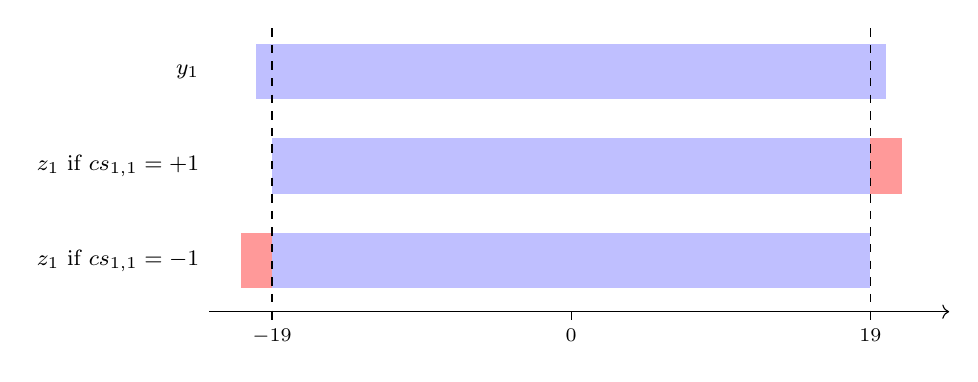
\begin{tikzpicture}[x=0.2cm,y=1cm]
\fill[blue!25] (-20,0) rectangle (20,0.7);
\node[anchor=east,font=\footnotesize] at (-23,0.35) {$y_1$};
\fill[blue!25] (-19,-1.2) rectangle (19,-0.5);
\fill[red!40] (19,-1.2) rectangle (21,-0.5);
\node[anchor=east,font=\footnotesize,align=right] at (-23,-0.85) {$z_1$ if $cs_{1,1}=+1$};
\fill[blue!25] (-19,-2.4) rectangle (19,-1.7);
\fill[red!40] (-21,-2.4) rectangle (-19,-1.7);
\node[anchor=east,font=\footnotesize,align=right] at (-23,-2.05) {$z_1$ if $cs_{1,1}=-1$};
\draw[dashed] (-19,0.9) -- (-19,-2.7);
\draw[dashed] (19,0.9) -- (19,-2.7);
\draw[->] (-23,-2.7) -- (24,-2.7);
\foreach \x in {-19,0,19}{\draw (\x,-2.7) -- (\x,-2.8) node[below,font=\scriptsize] {$\x$};}
\end{tikzpicture}
\caption{Rejection sampling for one coordinate. The mask $y_1$ is uniform on $[-20,20]$. Shifting by $cs_{1,1}=\pm1$ moves the range, and the red parts exist for only one sign. Rejecting every $z_1$ outside $[-19,19]$ discards the red parts and leaves the same uniform distribution for both signs.}
\end{figure}

The price is that signing sometimes fails and has to be repeated. In the real schemes the parameters are tuned so that the expected number of attempts is small (about four to five for ML-DSA), and the rejected attempts are never output.

\begin{figure}[h]
\centering
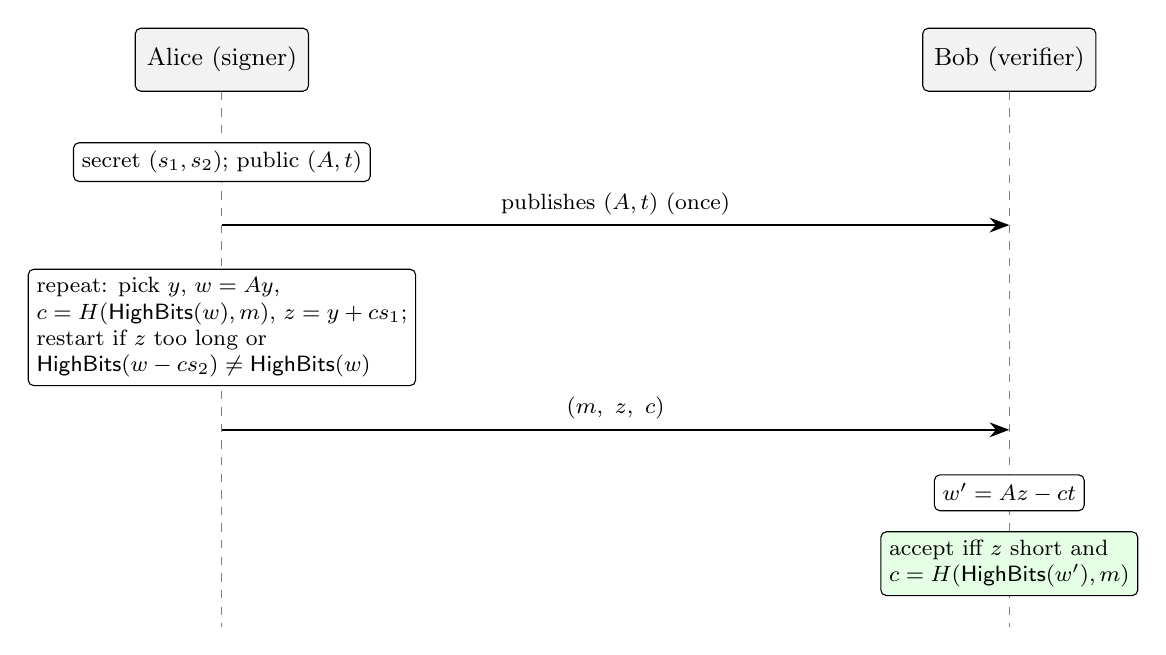
\begin{tikzpicture}[x=1cm,y=1cm]
\node[actor] (A) at (0,0) {Alice (signer)};
\node[actor] (B) at (10,0) {Bob (verifier)};
\draw[life] (A) -- (0,-7.2); \draw[life] (B) -- (10,-7.2);
\node[box,align=left] at (0,-1.3) {secret $(s_1,s_2)$;\ public $(A,t)$};
\draw[msg] (0,-2.1) -- (10,-2.1) node[midway,above,font=\footnotesize] {publishes $(A,t)$ (once)};
\node[box,align=left] at (0,-3.4) {repeat: pick $y$, $w=Ay$,\\$c=\Hash(\HB(w),m)$, $z=y+cs_1$;\\restart if $z$ too long or\\$\HB(w-cs_2)\ne\HB(w)$};
\draw[msg] (0,-4.7) -- (10,-4.7) node[midway,above,font=\footnotesize] {$(m,\ z,\ c)$};
\node[box,align=left] at (10,-5.5) {$w'=Az-ct$};
\node[box,fill=green!10,align=left] at (10,-6.4) {accept iff $z$ short and\\$c=\Hash(\HB(w'),m)$};
\end{tikzpicture}
\caption{The interaction in a Fiat--Shamir-with-aborts signature. Alice's restarts are local and never seen by Bob.}
\end{figure}

\subsection{From the toy to ML-DSA and Falcon}

The toy scheme has the structure of ML-DSA, but the real scheme differs in scale and in a few details. The entries of $A,y,z,s_1,s_2$ are not integers but polynomials in the ring $R_q=\Z_q[X]/(X^{256}+1)$ with $q=8380417$, and $A$ is a $k\times\ell$ matrix of such polynomials (a module), where $(k,\ell)=(4,4),(6,5),(8,7)$ for the three security levels ML-DSA-44, ML-DSA-65 and ML-DSA-87. The challenge $c$ is a polynomial with exactly $\tau$ coefficients equal to $\pm1$ and all others zero ($\tau=39,49,60$ for the three levels), so that $cs_1$ stays short, and it is computed by hashing $\HB(w)$ together with a hash of the message. The public key is compressed by dropping the low-order bits of $t$, and the signature carries a small \emph{hint} that lets the verifier still recover $\HB(w)$ correctly. Security rests on Module-LWE (hiding $s_1,s_2$) and Module-SIS (preventing forgery).

\begin{table}[h]
\centering\footnotesize\setlength{\tabcolsep}{3.5pt}
\begin{tabular}{lllrrl}
\toprule
Scheme & Hard problem & Design & Public key & Signature & Quantum-safe\\
\midrule
RSA-3072 (PSS) & factoring / RSA & hash-and-sign & 384 B & 384 B & no\\
ECDSA, \texttt{secp256k1} & ECDLP & DSA-style & 33 B & 64 B (raw) & no\\
Schnorr (BIP~340) & ECDLP & Fiat--Shamir & 32 B & 64 B & no\\
ML-DSA-44 (Dilithium) & Module-LWE/SIS & Fiat--Shamir with aborts & 1312 B & 2420 B & yes\\
Falcon-512 & NTRU-SIS & hash-and-sign (GPV) & 897 B & about 666 B & yes\\
\bottomrule
\end{tabular}
\caption{Approximate key and signature sizes. Lattice signatures are roughly an order of magnitude larger than elliptic-curve ones, which is the main practical cost of post-quantum security, for instance in a blockchain where every transaction carries a signature.}\label{tab:sizes}
\end{table}

\subsection{Summary of the three families}

RSA signatures raise a hash to the secret power $d$, and verification raises the signature to the public power $e$; the trapdoor is knowing the factorization of $n$. Bitcoin's ECDSA and Schnorr signatures commit to a random point $R=kG$, bind it to the message and the public key through a hash, and respond with a value $s$ that mixes the nonce $k$ with the secret key $d$ linearly (Schnorr) or through an inverse (ECDSA); the trapdoor is the discrete logarithm problem on the curve. Lattice signatures either use a short basis as a trapdoor for CVP (hash-and-sign, with Gaussian sampling to hide the basis) or follow the Schnorr pattern with small vectors and rejection sampling (Fiat--Shamir with aborts); their security comes from LWE and SIS. All three obey the same interface $(\Gen,\Sign,\Ver)$ from Section~0, all three hash the message before using it, and the first two are broken by a quantum computer while the third is believed to resist it.

%=====================================================================
\section{Certificates and the TLS Handshake}
%=====================================================================

\subsection{The binding problem}

A signature proves that whoever holds a secret key signed a message. It does not say who that person is. When Bob receives a public key together with the claim ``this is Alice's key'', the claim itself carries no proof. If Oscar can slip his own public key to Bob under Alice's name, then every signature that Oscar makes will verify as ``Alice's'' signature. The signature schemes of Sections~1 to~3 are therefore only as trustworthy as the way public keys are delivered.

One solution is to meet in person and exchange keys, which works for a handful of friends and not for a web browser that visits thousands of sites. The solution used in practice is to let a trusted party vouch for the binding between a name and a key, by signing it.

\subsection{Certificates}

\begin{definition}[Certificate]
A \emph{certificate} is a signed statement from a \emph{certificate authority} (CA) of the form
\[
\mathrm{Cert}_A=\big(\ \text{identity},\ \pk_A,\ \text{validity period},\ \sigma_{\mathrm{CA}}\ \big),\qquad \sigma_{\mathrm{CA}}=\Sign\big(\sk_{\mathrm{CA}},\ (\text{identity},\pk_A,\text{validity})\big).
\]
Anybody who knows the CA's public key $\pk_{\mathrm{CA}}$ can verify the certificate and then trust that $\pk_A$ belongs to the named identity, to the extent that the CA checked this before signing.
\end{definition}

In plain words, a certificate is a signature used as a name tag. Bob no longer has to trust Alice's key directly. He has to trust the CA's key, which his browser or operating system ships with, and the CA's signature carries the trust over to Alice's key.

\begin{example}[Alice's certificate]\label{ex:cert}
Let the CA have the RSA key pair $p=47$, $q=59$, so $n_{\mathrm{CA}}=2773$ and $\varphi=46\cdot 58=2668$. With $e_{\mathrm{CA}}=17$ the secret exponent is $d_{\mathrm{CA}}=157$, since $17\cdot 157=2669=2668+1$. Alice's own key from Example~\ref{ex:rsakey} is $(n_A,e_A)=(3233,17)$.

Alice asks the CA for a certificate. After checking her identity the CA writes the statement $\mathrm{tbs}=\text{``ALICE;3233;17''}$ (the ``to be signed'' part), hashes it with the toy hash from before, now reduced modulo $2773$, and signs it. The ASCII codes add up to $775$, so $h=775$, and
\[
\sigma_{\mathrm{CA}}=775^{157} \bmod 2773=2193.
\]
The certificate is $(\text{``ALICE;3233;17''},\ 2193)$.

Bob receives it from Alice's server. He hashes the statement to obtain $h=775$ and computes $2193^{17} \bmod 2773=775$. The values agree, so Bob accepts that the key $(3233,17)$ belongs to Alice.
\end{example}

\begin{example}[A forged certificate is rejected]\label{ex:certforge}
Oscar takes Alice's certificate and replaces her modulus by his own, producing the statement $\text{``ALICE;3229;17''}$ with the same signature $2193$. Bob hashes the statement and gets $780$, but the signature produces $2193^{17} \bmod 2773=775$. Since $775\ne 780$, Bob rejects. To make a fake certificate pass, Oscar would have to produce a value $s'$ with $s'^{17}\equiv 780 \pmod{2773}$, which requires the CA's secret exponent.
\end{example}

\subsection{Chains of trust}

A browser cannot hold the public key of every website's CA, and a CA's most valuable key should rarely be used. The solution is a chain. A \emph{root CA} has a self-signed certificate that is installed in the browser or operating system and is trusted without any signature to check. The root key is kept offline and is used only to sign the certificates of a few \emph{intermediate CAs}. An intermediate CA signs certificates for websites. When a server connects it sends its own certificate together with the intermediate certificate, and the browser verifies the chain upwards.

\begin{figure}[h]
\centering
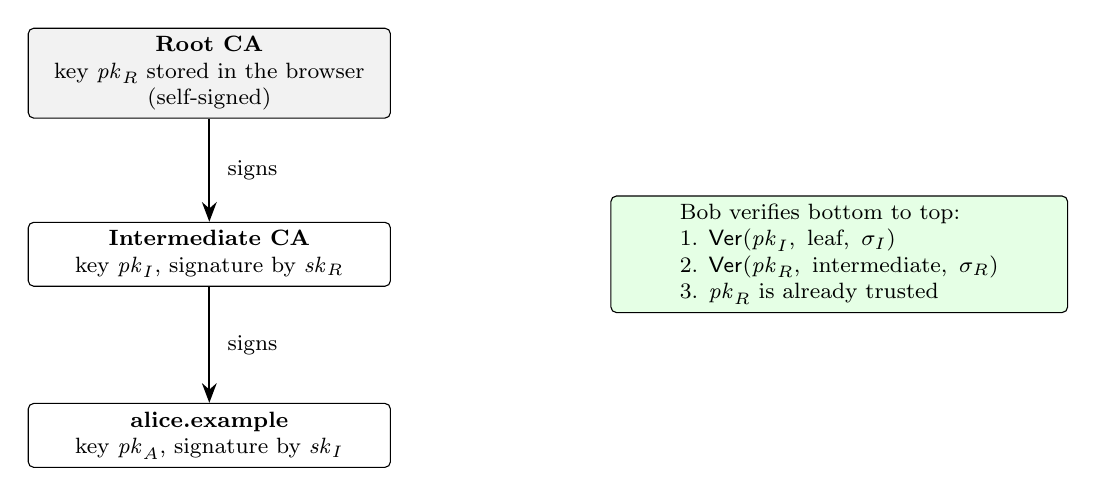
\begin{tikzpicture}[x=1cm,y=1cm]
\node[box,align=center,minimum width=4.6cm,fill=gray!10] (root) at (0,0) {\textbf{Root CA}\\key $\pk_R$ stored in the browser\\(self-signed)};
\node[box,align=center,minimum width=4.6cm] (int) at (0,-2.3) {\textbf{Intermediate CA}\\key $\pk_I$, signature by $\sk_R$};
\node[box,align=center,minimum width=4.6cm] (leaf) at (0,-4.6) {\textbf{alice.example}\\key $\pk_A$, signature by $\sk_I$};
\draw[msg] (root) -- (int) node[midway,right,font=\footnotesize] {\ signs};
\draw[msg] (int) -- (leaf) node[midway,right,font=\footnotesize] {\ signs};
\node[box,align=left,fill=green!10,minimum width=5.8cm] at (8,-2.3) {Bob verifies bottom to top:\\1. $\Ver(\pk_I,\ \text{leaf},\ \sigma_I)$\\2. $\Ver(\pk_R,\ \text{intermediate},\ \sigma_R)$\\3. $\pk_R$ is already trusted};
\end{tikzpicture}
\caption{A chain of trust. The server sends the two lower certificates, and the browser supplies the root key from its own trust store.}\label{fig:chain}
\end{figure}

\begin{definition}[Validating a chain]
Bob accepts $\pk_A$ for the name \texttt{alice.example} if (i)~the leaf certificate names \texttt{alice.example} and is within its validity period, (ii)~each certificate in the chain is correctly signed by the key in the certificate above it, and (iii)~the top of the chain is a root key that Bob already trusts.
\end{definition}

In the chain of Figure~\ref{fig:chain} there are two signature verifications, and each of them is an ordinary run of $\Ver$ from Section~0. Any of the three families of the previous sections can be used for any link.

\subsection{When the chain breaks}

Trust in a chain is exactly as strong as its weakest CA. If a CA signs a certificate for \texttt{alice.example} without checking the requester, or if its signing key is stolen, then Oscar holds a perfectly valid certificate for Alice's name and the verification of Example~\ref{ex:cert} succeeds for him. This has happened to real CAs, which is why browsers distrust CAs that misbehave and why certificates are logged in public \emph{certificate transparency} logs, where domain owners can look for certificates they did not request. A certificate also has a limited validity period, of at most about a year, so that a leaked private key stops being useful after a bounded time. A certificate whose key is known to be stolen can be revoked before it expires, through lists published by the CA or through online status checks, which browsers consult with varying strictness.

\begin{remark}[Bitcoin has no certificates]
The Bitcoin network avoids the binding problem by removing identities. A public key is itself the owner, and an address is a hash of it. A transaction proves that its sender holds the secret key for a given address, and nobody needs to know the person behind it. A web server has the opposite requirement: the browser must know that it is talking to the owner of a particular \emph{name}, and a certificate is how a name is connected to a key.
\end{remark}

\subsection{The TLS 1.3 handshake}\label{sec:tls}

TLS is the protocol behind every \texttt{https} connection. Its handshake combines three tools from these notes. A key exchange (Diffie--Hellman) lets the two sides agree on a secret over an open channel, signatures and certificates authenticate the server, and a MAC confirms that both sides saw the same handshake. Encryption, which was the starting point of Section~0, comes only afterwards and uses the agreed secret.

\emph{Key exchange.} In the ephemeral Diffie--Hellman variant (ECDHE) Bob, the client, picks a fresh secret $a$ and sends $A=aG$. The server Alice picks a fresh secret $b$ and sends $B=bG$. Both compute the same shared point $S=aB=bA=abG$ and derive their session keys from it. The numbers $a$ and $b$ are thrown away after the handshake. A key exchange alone does not authenticate anybody, because Oscar could run one exchange with Bob and another with Alice.

\emph{Authentication.} After the key shares, the server sends its certificate chain and a message called \texttt{CertificateVerify}. It contains a signature, made with the secret key that belongs to the certified public key, over a hash of the whole handshake so far, including both key shares. Bob verifies the chain and then the signature. A valid signature shows that the party that sent $B$ holds the secret key for the certified name, and it also shows that $A$ and $B$ were not altered on the way.

\emph{Confirmation.} Finally each side sends a \texttt{Finished} message, a MAC over the transcript computed with a key derived from $S$, which proves that it computed the same shared secret and saw the same handshake.

\begin{figure}[h]
\centering
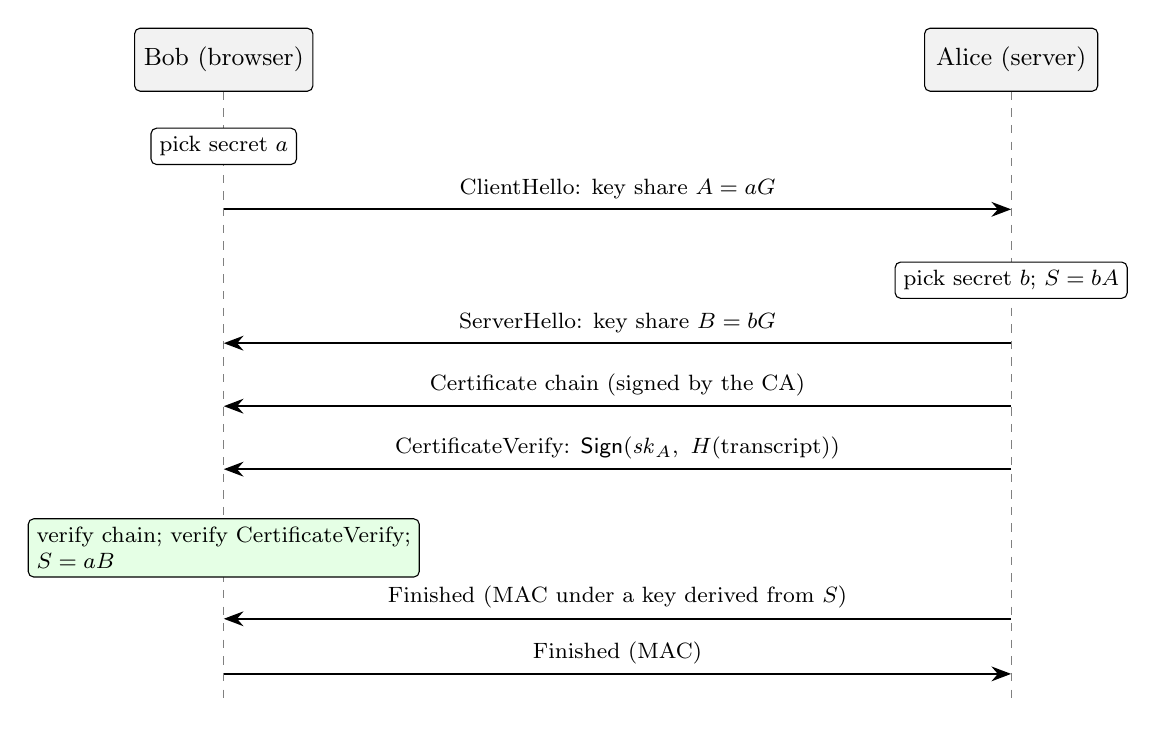
\begin{tikzpicture}[x=1cm,y=1cm]
\node[actor] (B) at (0,0) {Bob (browser)};
\node[actor] (A) at (10,0) {Alice (server)};
\draw[life] (B) -- (0,-8.2); \draw[life] (A) -- (10,-8.2);
\node[box,align=left] at (0,-1.1) {pick secret $a$};
\draw[msg] (0,-1.9) -- (10,-1.9) node[midway,above,font=\footnotesize] {ClientHello: key share $A=aG$};
\node[box,align=left] at (10,-2.8) {pick secret $b$;\ $S=bA$};
\draw[msg] (10,-3.6) -- (0,-3.6) node[midway,above,font=\footnotesize] {ServerHello: key share $B=bG$};
\draw[msg] (10,-4.4) -- (0,-4.4) node[midway,above,font=\footnotesize] {Certificate chain (signed by the CA)};
\draw[msg] (10,-5.2) -- (0,-5.2) node[midway,above,font=\footnotesize] {CertificateVerify: $\Sign(\sk_{A},\ \Hash(\text{transcript}))$};
\node[box,align=left,fill=green!10] at (0,-6.2) {verify chain;\ verify CertificateVerify;\\$S=aB$};
\draw[msg] (10,-7.1) -- (0,-7.1) node[midway,above,font=\footnotesize] {Finished (MAC under a key derived from $S$)};
\draw[msg] (0,-7.8) -- (10,-7.8) node[midway,above,font=\footnotesize] {Finished (MAC)};
\end{tikzpicture}
\caption{The TLS 1.3 handshake, reduced to the messages that matter here. Key exchange gives secrecy, the certificate and the signature give authentication, and the \texttt{Finished} MACs confirm both sides agree.}
\end{figure}

\begin{example}[A handshake with small numbers]\label{ex:tls}
Use the curve of Example~\ref{ex:curve} with $G=(2,12)$ and the order $31$, and let Alice's server use the RSA key $(n,e,d)=(3233,17,2753)$ from Example~\ref{ex:rsakey}, certified in Example~\ref{ex:cert}.

Bob picks $a=4$ and sends $A=4G=(21,18)$. Alice picks $b=9$ and sends $B=9G=(20,40)$. Bob computes $S=aB=4\cdot 9G=36G=5G=(12,12)$ (since $36=31+5$), and Alice computes $S=bA=9\cdot 4G=36G=(12,12)$. Both hold the same secret point.

The transcript is the string $\text{``21,18|20,40''}$. With the toy hash (sum of ASCII codes modulo $3233$) it hashes to $t=614$. Alice's \texttt{CertificateVerify} is
\[
\sigma=614^{2753} \bmod 3233=1198.
\]
Bob has already validated Alice's certificate and therefore trusts the key $(3233,17)$. He recomputes the transcript hash $614$ from the key shares he sent and received, and checks $1198^{17} \bmod 3233=614$. The values agree, so he knows that the sender of $B$ is the holder of the certified key and that the key shares are the ones in the signed transcript.
\end{example}

\begin{example}[Why the signature stops a man-in-the-middle]\label{ex:mitm}
Oscar sits between Bob and Alice. He lets $A=(21,18)$ reach Alice, but he replaces Alice's key share by his own $B'=6G=(29,31)$ so that he can agree on a secret with Bob. He cannot create a signature for a transcript containing $B'$, since he does not have $d=2753$. The best he can do is forward Alice's genuine certificate chain and her genuine \texttt{CertificateVerify} value $1198$.

Bob's transcript now reads $\text{``21,18|29,31''}$ and its hash is $t'=623$. He computes $1198^{17} \bmod 3233=614\ne 623$ and aborts the handshake. A plain Diffie--Hellman exchange with no signature would have gone through without any warning, and Oscar would have been able to read and modify the whole connection.
\end{example}

\begin{example}[Forward secrecy]\label{ex:fs-tls}
Suppose Oscar records the whole conversation of Example~\ref{ex:tls}, including $A=(21,18)$ and $B=(20,40)$, and a year later steals Alice's long-term key $d=2753$. The secret $S=abG$ cannot be recomputed from this: the signing key was used only to authenticate, and it contains no information about $a$ or $b$. Oscar would have to solve a discrete logarithm problem, finding $a$ from $A=aG$ or $b$ from $B=bG$. On this toy curve that is a table lookup, and on \texttt{secp256k1}-sized curves it is infeasible. This property is called \emph{forward secrecy}.

Older TLS 1.2 deployments could instead let Bob encrypt a random secret directly to the server's RSA key. In that mode a recorded session is decrypted as soon as the server key is stolen, which is why TLS 1.3 removed it.
\end{example}

\subsection{Signature sizes in certificate chains}

A TLS handshake with the chain of Figure~\ref{fig:chain} carries three signatures: the one on the leaf certificate, the one on the intermediate certificate, and \texttt{CertificateVerify}, together with two certified public keys. With elliptic-curve signatures of roughly $70$ bytes and keys of $65$ bytes, this adds up to about $350$ bytes. With ML-DSA-44 from Table~\ref{tab:sizes} (signatures of $2420$ bytes and public keys of $1312$ bytes) it is about $3\cdot 2420+2\cdot 1312\approx 9.9$ kilobytes. Large handshakes cost time on slow connections, which is a practical reason why replacing the signatures in certificate chains by post-quantum ones is a difficult engineering problem, in addition to the mathematical one of Section~3.

\end{document}
